
\documentclass[xcolor={dvipsnames}]{beamer}
\usepackage{amsmath}
% \usepackage{beamerthemesplit} // Activate for custom appearance
\usepackage{hyperref}
\usepackage{ragged2e}
\usepackage{amssymb}
\usepackage{verbatim}
\usepackage{lmodern}



\title{Regression}
\author{Schwartz}
\date{\today}



\begin{document}




\frame{\titlepage}




\frame
{
 \frametitle{The Sophomore Slump}

{
\fontfamily{<familyname>}\selectfont
\begin{quote}
\tiny
\justify

...or \emph{$sophomore$ $jinx$} or \emph{$sophomore$ $jitters$} refers to an instance in which a second, or sophomore, effort fails to live up to the standards of the first effort. It is commonly used to refer to the apathy of students (second year of high school, college or university), the performance of athletes (second season of play), singers/bands (second album), television shows (second seasons) and films (sequels/prequels). In the United Kingdom the \emph{$sophomore$ $slump$} is more commonly referred to as \emph{$second$ $year$ $blues$}, particularly when describing university students. And in Australia it is known as \emph{$second$ $year$ $syndrome$}, and is particularly common when referring to professional athletes who have a mediocre second season following a stellar debut. The phenomenon of a \emph{sophomore slump} can be explained psychologically, where earlier success has a reducing effect on the subsequent effort, but it can also be explained statistically, as an effect of the regression towards the mean.

\end{quote}
}

\begin{columns}
\begin{column}{.011\textwidth}
\end{column}
\begin{column}{.6\textwidth}
{
\fontfamily{<familyname>}\selectfont
\begin{quote}
\tiny
\justify

The concept of $regression$ comes from genetics and was popularized by Sir Francis Galton's late 19th century publication of ``Regression towards mediocrity in hereditary stature.'' Galton observed that extreme characteristics (e.g., height) in parents are not completely passed on to offspring, but rather the characteristics in the offspring ``regress'' towards a mediocre point. By measuring the heights of hundreds of people Galton was able to quantify this ``regression'' and in so doing invented linear regression analysis, thus laying the groundwork for much of modern statistical modeling. The term $regression$ stuck.
\end{quote}
}
\end{column}
\begin{column}{.4\textwidth}
\vspace{.1in}
\hspace*{-.39in}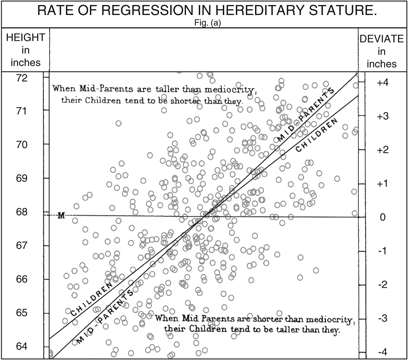
\includegraphics[width=1.55in]{stuff/galton.jpg} 

\end{column}
\end{columns}

% that the offspring of parents who lie at the tails of the distribution will tend to lie closer to the mean of the distribution. 

}



\frame
{
\normalsize
 \frametitle{Objectives}
\begin{itemize}
\item Linear Model Regression 
\begin{itemize}
\item Terminology 
\item \textcolor{gray}{Model Fitting (Least Squares)} 
\item Diagnostics (Evaluation and Critiquing) 
\end{itemize}
\item Multiple (not Multivariate) Linear Regression
\begin{itemize}
\item \textcolor{gray}{Assumptions}
\item \textcolor{gray}{Normal Distribution Theory}  
\item Model Selection
\item Coefficient Testing
\end{itemize}
\item \textcolor{gray}{Alternatives to linear forms}
%\item \textcolor{gray}{Demo}
\end{itemize}

}



\definecolor{aliceblue}{rgb}{.64,.77,.95}
\frame
{
 \frametitle{Linear Models and Regression Terminology}


\vspace{-.25em}
\begin{itemize}
\item[]<2->\textcolor{red}{Outcome / Response / Label / Dependent/Endogenous Var.}
\item $\only<1>{Y_i}\only<2->{\textcolor{red}{Y_i}} = \beta_0  +   \only<1-2>{x_i}\only<3->{\textcolor{blue}{x_i}}\beta_1 + \epsilon_i, \epsilon_i \overset{\tiny i.i.d.}{\sim}  Normal(0,\sigma^2)$
\item[]<3->  \hspace{4.1em}  \textcolor{blue}{Feature / Covariate / Independent/Exogenous Var.}
\item[]<4->  \hspace{4.1em}   \textcolor{aliceblue}{ I don't like to call these \emph{Predictors}...}
\vspace{30em}${}$\\

\end{itemize}

}


\frame
{
 \frametitle{Linear Models and Regression Terminology}

\vspace{-1.05in}


\begin{itemize}
\item[]<2-> \hspace{4.85em}   \textcolor{orange}{Coefficient} 
\item $Y_i = \textcolor{purple}{\beta_0} + x_i\only<1>{\beta_1}\only<2->{\textcolor{orange}{\beta_1}} + \only<1-2>{\epsilon_i}\only<3->{\textcolor{brown}{\epsilon_i}}, \epsilon_i \overset{\tiny i.i.d.}{\sim}  Normal(0,\sigma^2)$
\item[]<1->  \hspace{1.85em}  \textcolor{purple}{Intercept}   \hspace{.85em} \only<3->{\textcolor{brown}{Error/Noise}}\\${}$\\

\vspace{-1em}
\onslide<4->{\includegraphics[width=3.5in]{stuff/Regression1.png}}

\item[]<6-> \textcolor{green}{Fitted/Predicted value $\hat Y_i$} $\quad$ \only<8->{\textcolor{blue}{Residual Variance}}
\item<5-> $\only<1-5>{Y_i = \hat\beta_0  +  x_i\hat\beta_1}  \only<6>{\textcolor{green}{\hat Y_i = \hat\beta_0  +  x_i\hat\beta_1}}  \only<7->{Y_i = \textcolor{green}{\hat\beta_0  +  x_i\hat\beta_1}} + \only<7->{\textcolor{red}{\hat \epsilon_i}}\only<1-6>{\hat \epsilon_i}, \quad \only<1-7>{\hat \sigma^2 = \frac{\sum_{i=1}^n \hat \epsilon_i^2}{n-p-1}}\only<8>{\textcolor{blue}{\hat \sigma^2 = \frac{\sum_{i=1}^n \hat \epsilon_i^2}{n-p-1}}}\only<9>{\textcolor{blue}{\hat \sigma^2 = \frac{\sum_{i=1}^n \hat \epsilon_i^2}{n-\textcolor{red}{\boldsymbol P-1}}}}  \quad (p = \# of \; coefficients)$
\item[]<7->   \hspace{7.3em} \textcolor{red}{Residual }
\end{itemize}

\vspace{-2.42in}
\onslide<5->{\hspace{4.8em}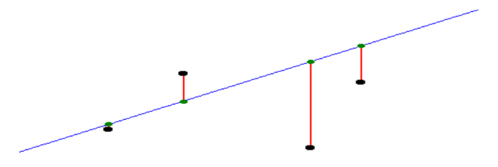
\includegraphics[width=2.76in,height=1.0in]{stuff/fit1.png}}

}


\frame
{
 \frametitle{Quiz: what are these things and their parts?}
 \huge
$$ Y_i = \beta_0 + x_i \beta_1 + \epsilon_i $$

$$ Y_i = \hat \beta_0 + x_i \hat \beta_1 + \hat \epsilon_i, \quad \hat \sigma^2 = \frac{\sum_{i=1}^n \hat \epsilon_i}{n-p-1}$$

$$ \hat Y_i = \hat \beta_0 + x_i \hat \beta_1 $$

}

\frame
{
 \frametitle{Least Squares Fit}

\begin{itemize}

\item $ Y_i = \hat\beta_0 + x_i\hat\beta_1 + \hat \epsilon_i$
\item[] 
\item[]<2->  $[\hat \beta_0,\hat \beta_1] = \underset{[\beta_0, \beta_1]}{argmin} \sum_{i=1}^n \hat \epsilon_i^2 = 
\underset{{\boldsymbol\beta}}{argmin} \sum_{i=1}^n (Y_i - \textbf{x}_i^T{\boldsymbol\beta})^2$\\
\footnotesize
where $\textbf{x}_i^T = [1,x_i]$ and $\textbf{${\boldsymbol\beta}$} = \left[\begin{array}{c} \beta_0\\ \beta_1\end{array}\right]$

\item[]<3-> 
$$\sum_{i=1}^n ( Y_i - \textbf{x}_i^T{\boldsymbol\beta})^2 = (\textbf{Y} - \textbf{x}{\boldsymbol\beta})^T(\textbf{Y} - \textbf{x}{\boldsymbol\beta})$$

\footnotesize
where $\textbf{Y}^T =  [Y_1,Y_2,\cdots,Y_n]$ and $\textbf{x}^T =  \left[\begin{array}{cccc}1&1&\cdots&1\\x_1&x_2&\cdots&x_n \end{array}\right]$

\item[]<4-> \begin{align*}
%\frac{d}{d\hat{\boldsymbol\beta}}
\nabla_{{\boldsymbol\beta}} {} & {\boldsymbol\beta}^T(\textbf{x}^T\textbf{x}) {\boldsymbol\beta}  -2 \textbf{Y}^T \textbf{x}{\boldsymbol\beta}   + \textbf{Y}^T\textbf{Y}\\
=  {} &2 (\textbf{x}^T\textbf{x}) {\boldsymbol\beta}  - 2 \textbf{Y}^T\textbf{x} \quad\quad \textcolor{gray}{\text{(set to \textbf{0} to minimize)}}\\ 
\Longrightarrow {} & \hat{\boldsymbol\beta}  = (\textbf{x}^T\textbf{x})^{-1}  \textbf{x}^T\textbf{Y} \Longrightarrow 
\text{fitted values } \hat {\boldsymbol Y}  =  \textbf{x}\hat {\boldsymbol\beta}\\
& \quad\quad\quad\quad\quad\quad\quad\quad\quad\quad\quad\quad\quad\quad\quad   \hat {\boldsymbol Y}  =  \textbf{x}(\textbf{x}^T\textbf{x})^{-1}  \textbf{x}^T\textbf{Y}
\end{align*}

\end{itemize}
}



\frame
{
 \frametitle{Least Squares Fit \emph{bonus}}
 
 \vspace{.5em}
 
\begin{enumerate}
\item Maximum likelihood estimation (MLE)  \textcolor{gray}{$\iff$ to lease squares!}
\begin{align*}
{} & \underset{{\boldsymbol\beta}}{argmax} \prod_{i=1}^n \frac{1}{\sqrt{2\pi \sigma^2}} e^{-\frac{1}{2\sigma^2}(Y_i-\textbf{x}_i^T{\boldsymbol\beta})^2}\\
= {} & 
\underset{{\boldsymbol\beta}}{argmax} (2\pi \sigma^2)^{-\frac{n}{2}} e^{-\frac{1}{2\sigma^2}(\textbf{Y} - \textbf{x}{\boldsymbol\beta})^T(\textbf{Y} - \textbf{x}{\boldsymbol\beta})}\\
= {} & 
\underset{{\boldsymbol\beta}}{argmax} -\frac{n}{2}\log(2\pi \sigma^2) -\frac{1}{2\sigma^2}(\textbf{Y} - \textbf{x}{\boldsymbol\beta})^T(\textbf{Y} - \textbf{x}{\boldsymbol\beta})\\
= {} & 
\underset{{\boldsymbol\beta}}{argmin} (\textbf{Y} - \textbf{x}_i{\boldsymbol\beta})^T(\textbf{Y} - \textbf{x}{\boldsymbol\beta}) \quad \textcolor{gray}{\text{[same as least squares!!]}}
\end{align*} 
\item In simple linear regression the $\underset{{\boldsymbol\beta}}{argmin}  (\textbf{Y} - \textbf{x}{\boldsymbol\beta})^T(\textbf{Y} - \textbf{x}{\boldsymbol\beta})$ is
\begin{align*}
\hat \beta_0 = {}& \bar Y -  \hat \beta_1 \bar x \\
\hat \beta_1 = {}& \frac{\sum_{i=1}^n (Y_i - \bar Y) (x_i - \bar x)}{\sum_{i=1}^n (x_i - \bar x)^2} = \frac{R_{xY}S_Y}{S_x}\\
\end{align*}
\end{enumerate}
}


\frame
{
 \frametitle{What makes these data points ``unusual''?}

\begin{figure}
\centering
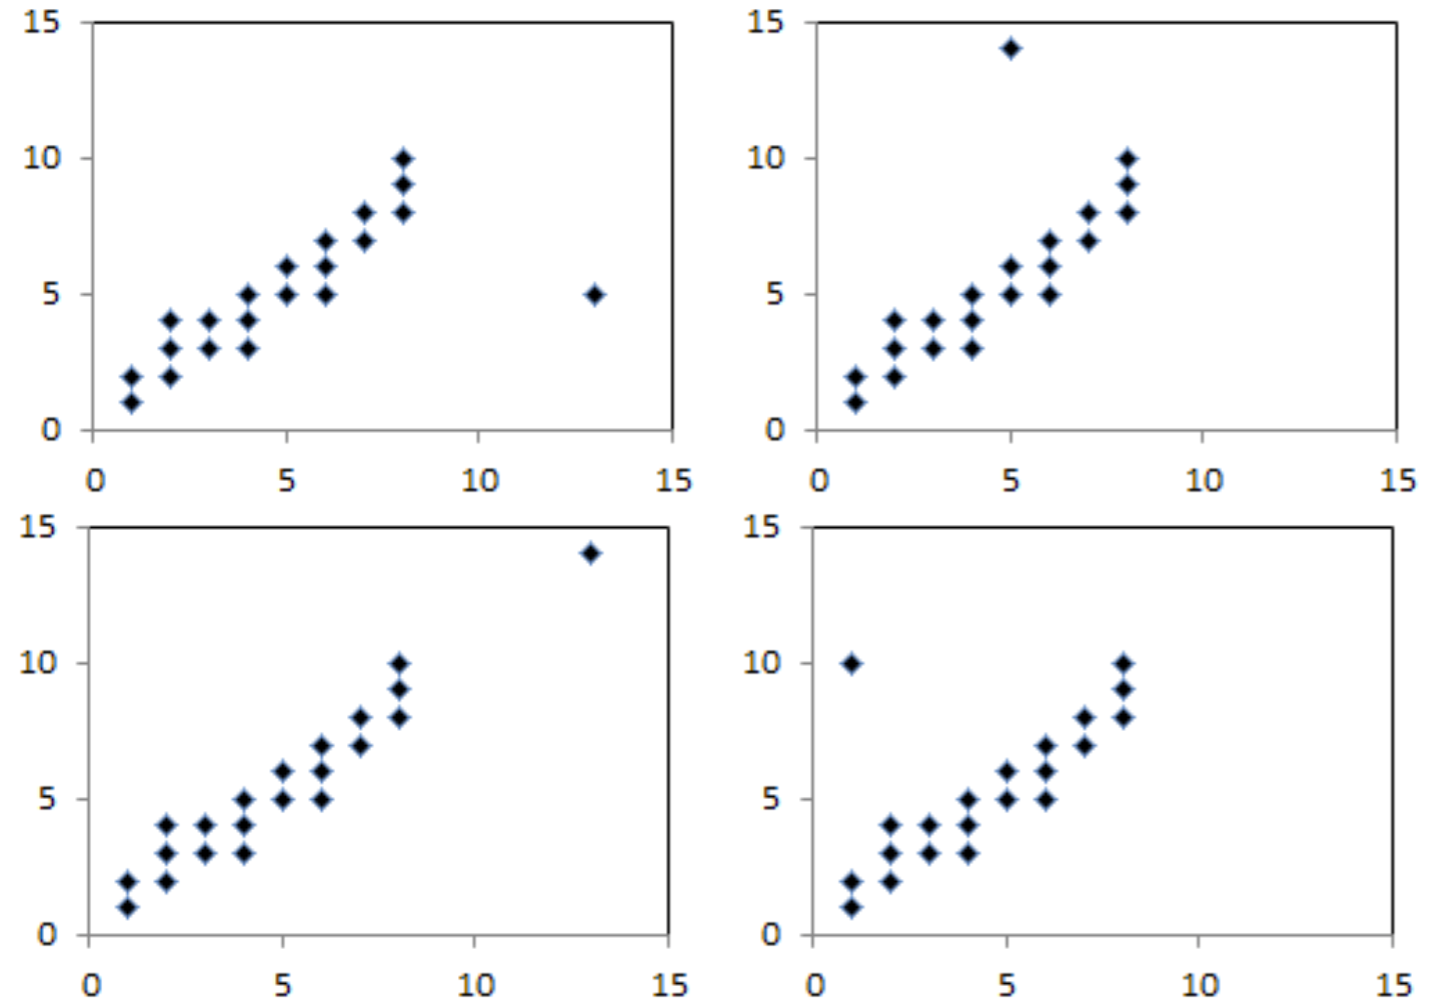
\includegraphics[width=4in]{stuff/outliers2.png}
\end{figure}
}


\frame
{
 \frametitle{Regression Diagnostics}

\vspace{.5em}
\emph{Outliers} \only<3->{{\textbf{\textcolor{blue}{impact residual variance estimates}}}}\\

\only<3->{\vspace{-.2em}}
\vspace{.5em}
\onslide<1->{\hspace{3em}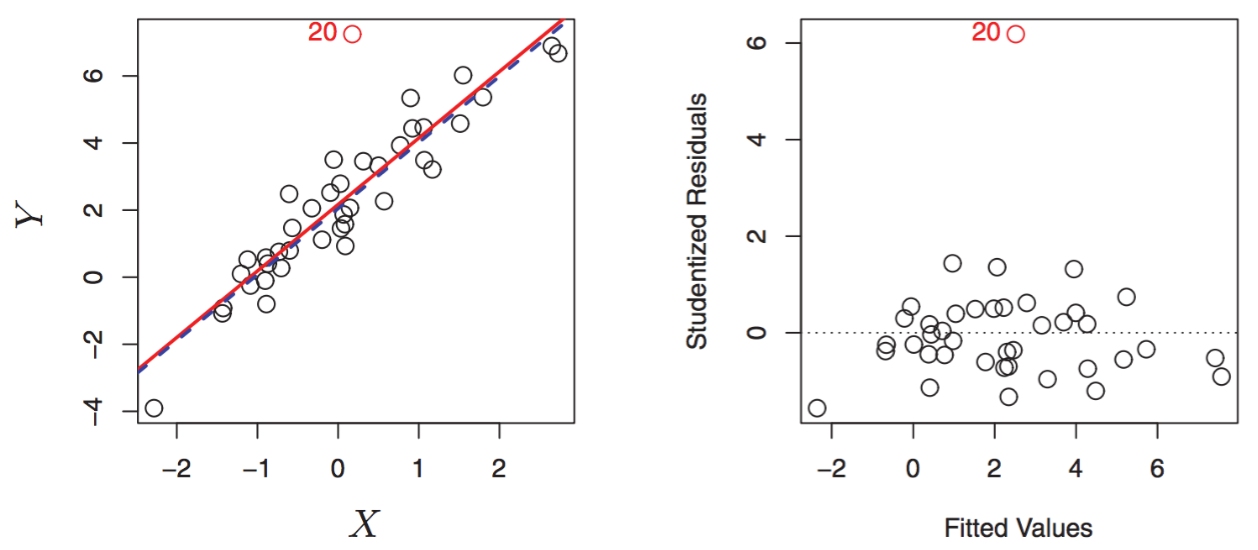
\includegraphics[height=1.4in]{stuff/outliers.png}}

\onslide<2->{\emph{High Leverage Points}} \only<3->{{\textbf{\textcolor{blue}{impact prediction estimates}}}}\\

\vspace{.5em}

\onslide<2->{\hspace{3em}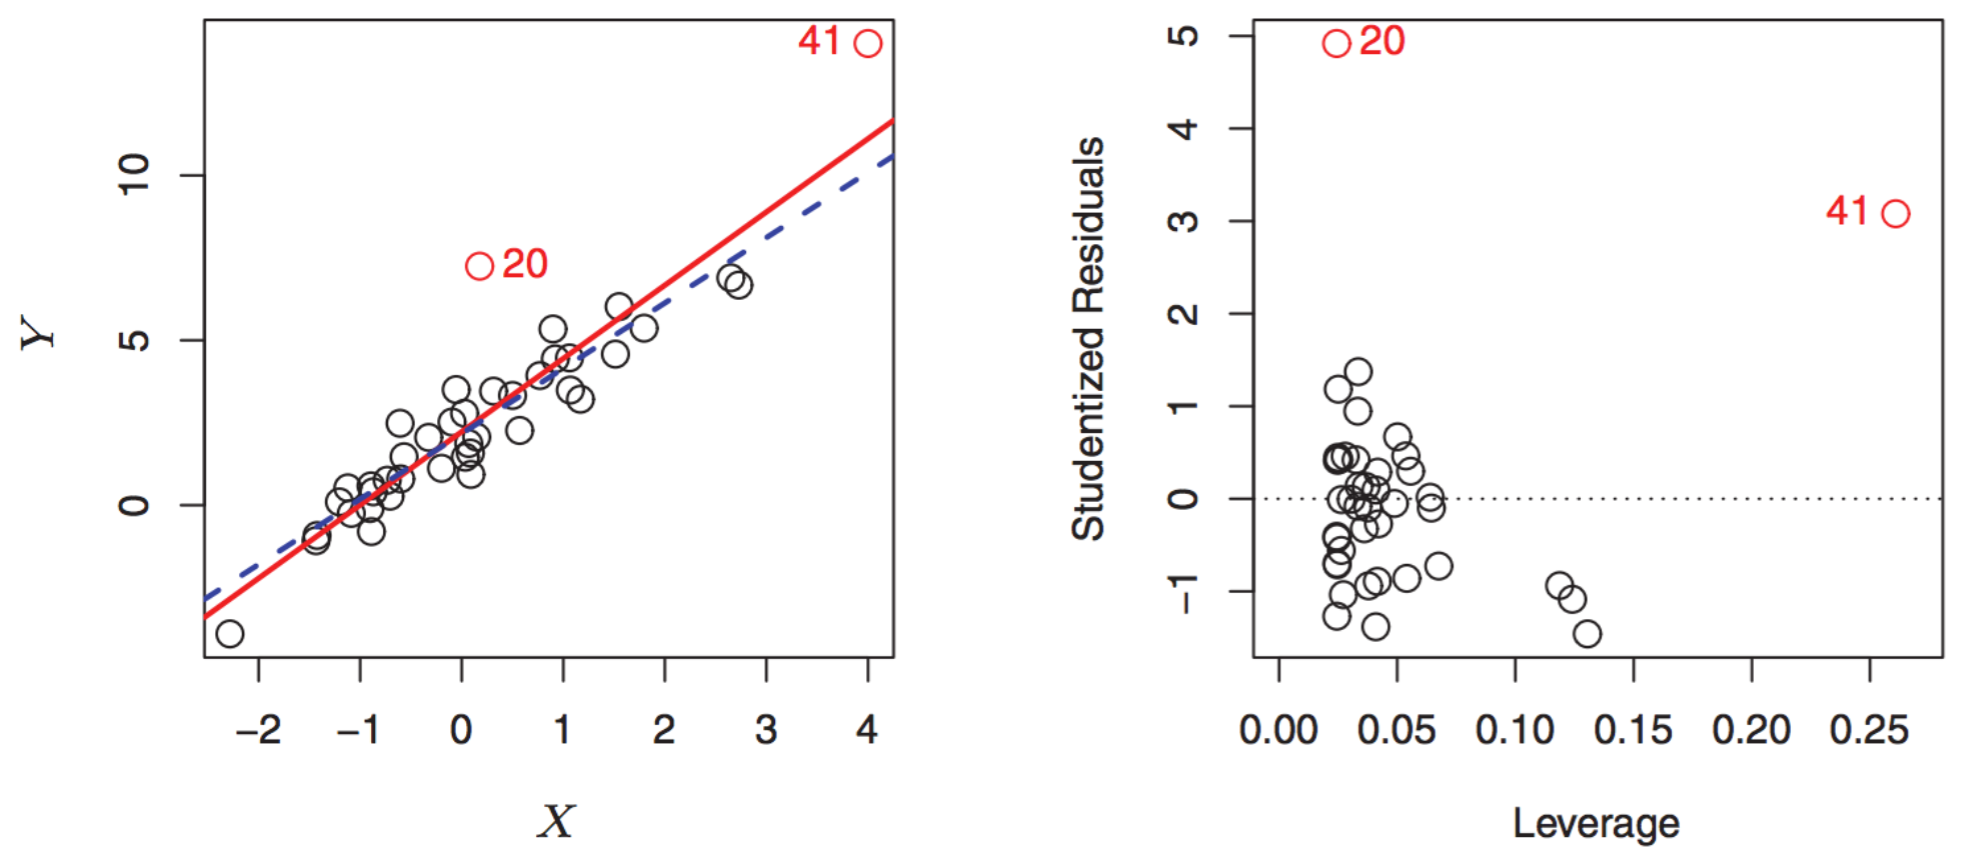
\includegraphics[height=1.41in]{stuff/outliers4.png}}

}

\frame
{
 \frametitle{Regression Diagnostics (with residuals)}

\only<1->{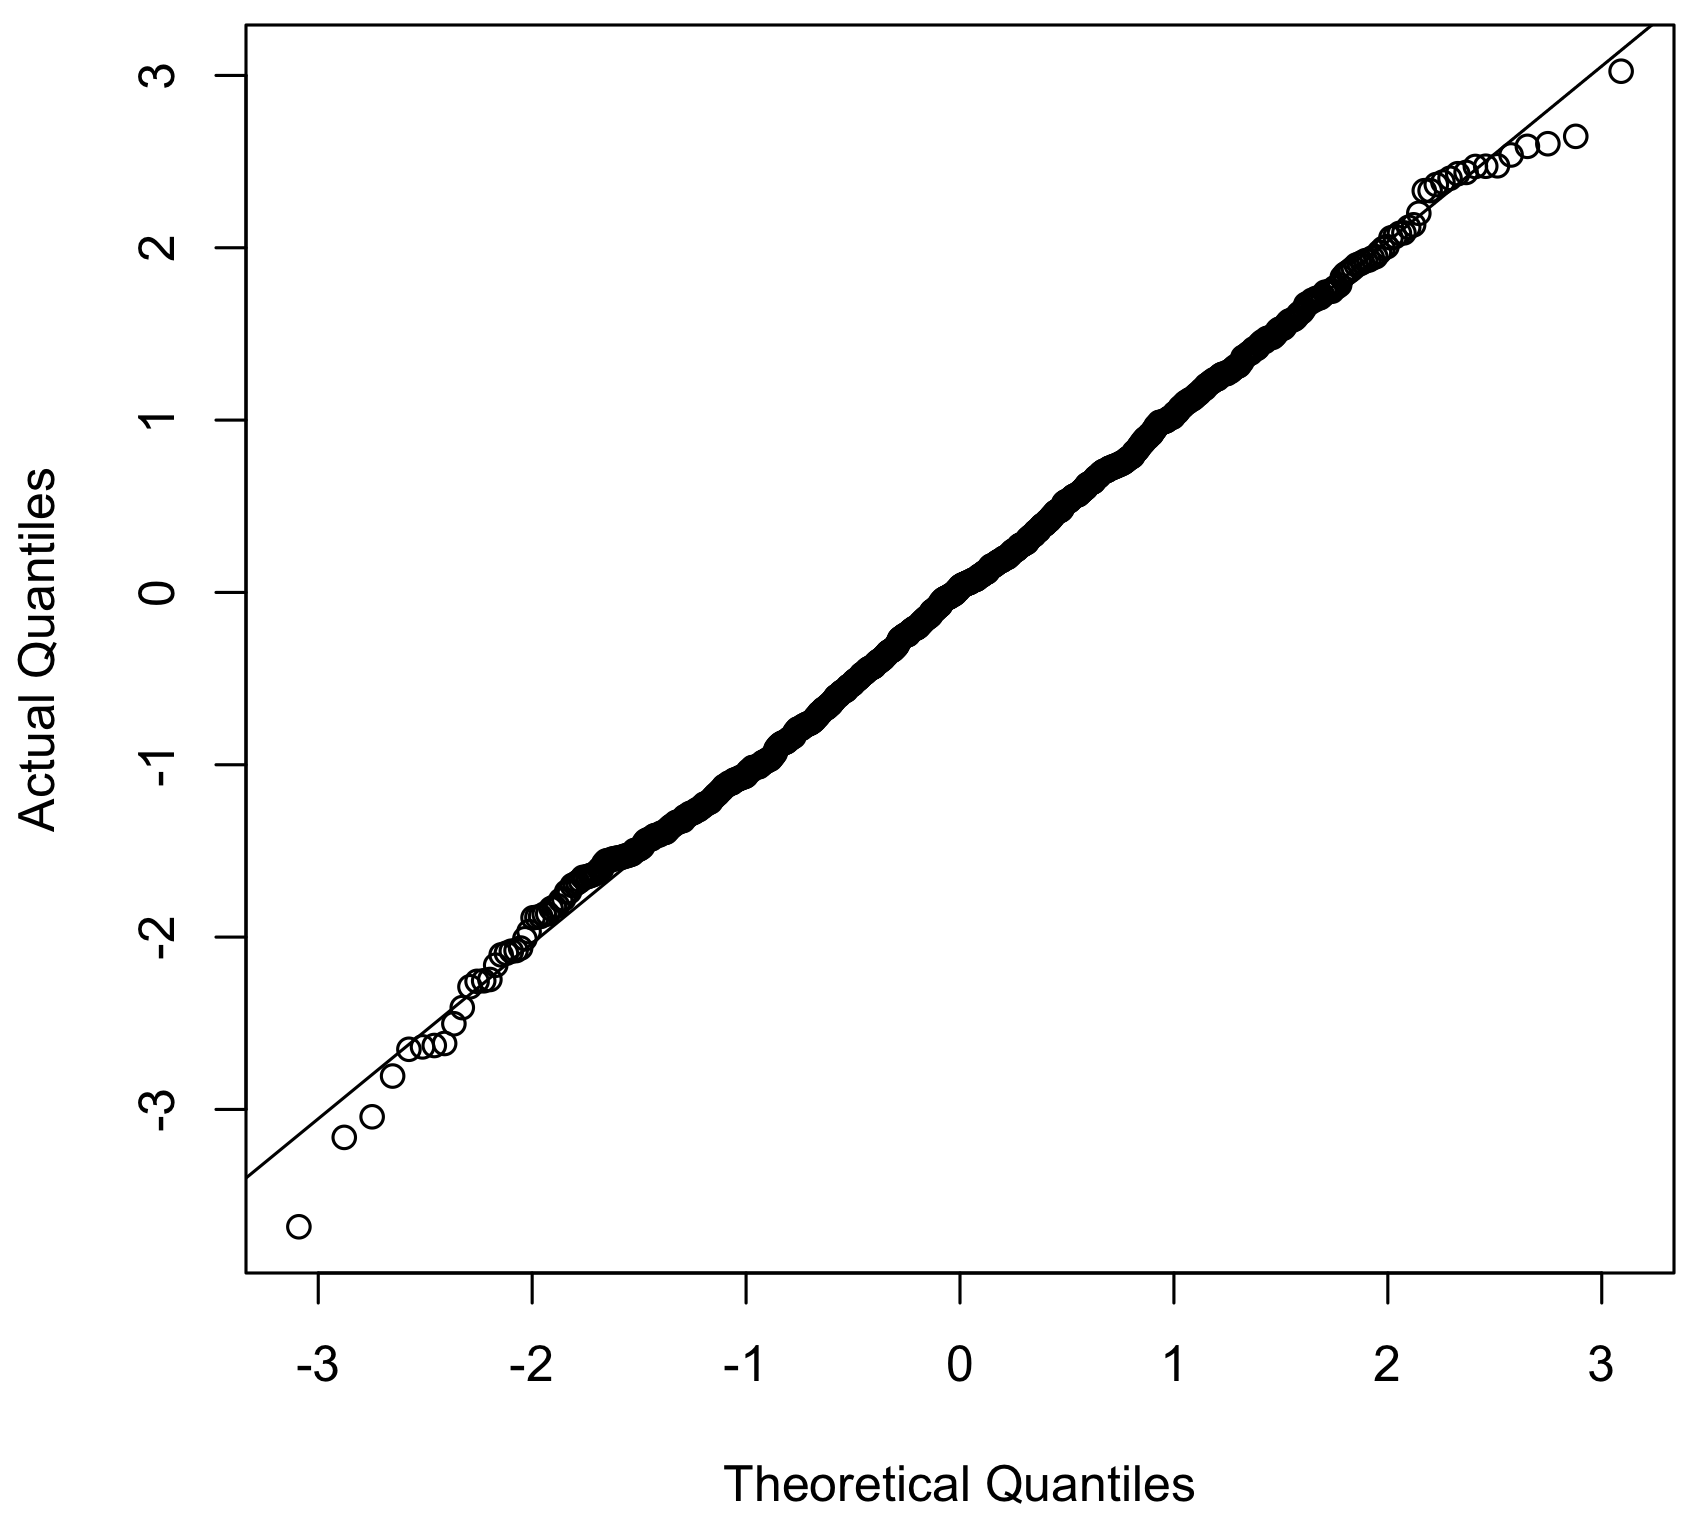
\includegraphics[width=1.75in]{stuff/qq1.png}}\only<1>{\hspace{-1.495in}\raisebox{.255in}{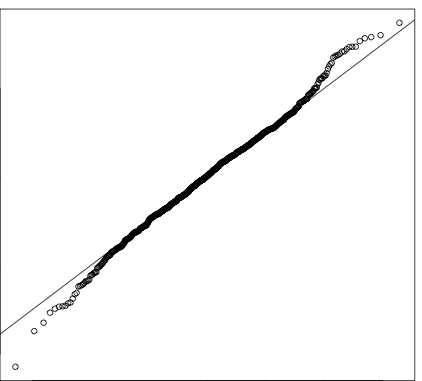
\includegraphics[width=1.495in, height=1.32in]{stuff/qq2.png}}}$\quad\quad\quad$\only<3>{\raisebox{-.1in}{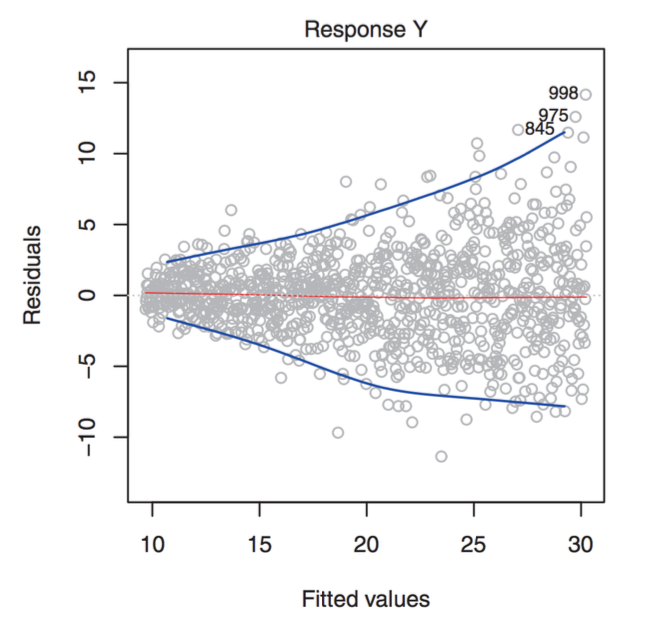
\includegraphics[width=1.825in]{stuff/hets1.png}}}\onslide<4->{\raisebox{-.1in}{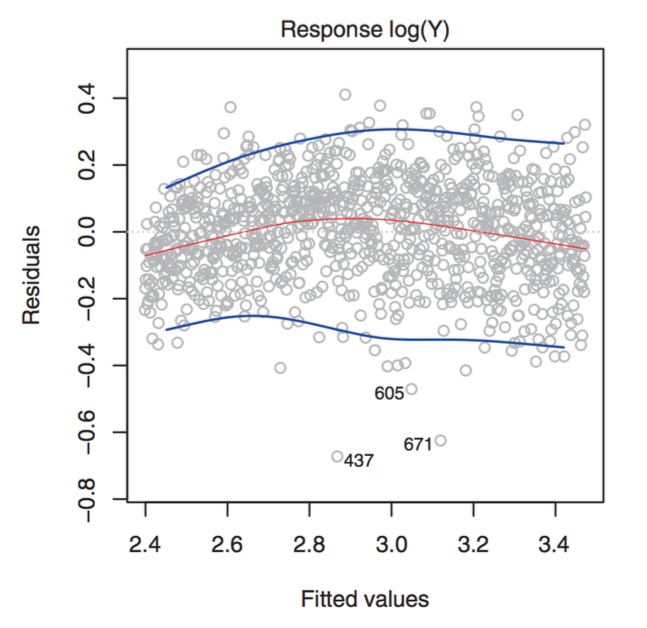
\includegraphics[width=1.825in]{stuff/hets2.png}}}

\vspace{-1.5in}$\quad\quad\;\;$QQ-plot

\vspace{1.35in}

\begin{columns}
\begin{column}{.4975\textwidth}
\vspace{-.5in}
\begin{itemize}
\setlength\itemsep{.75em}
\item<1-> What's wrong with the residual distribution?
\item<3-> \textcolor{NavyBlue}{What's wrong with the residual variance?}
\item<5-> \textcolor{red}{What's wrong with this $\text{feature/outcome relationship?}$}
\end{itemize}
\end{column}
\begin{column}{.5025\textwidth}
\onslide<5->{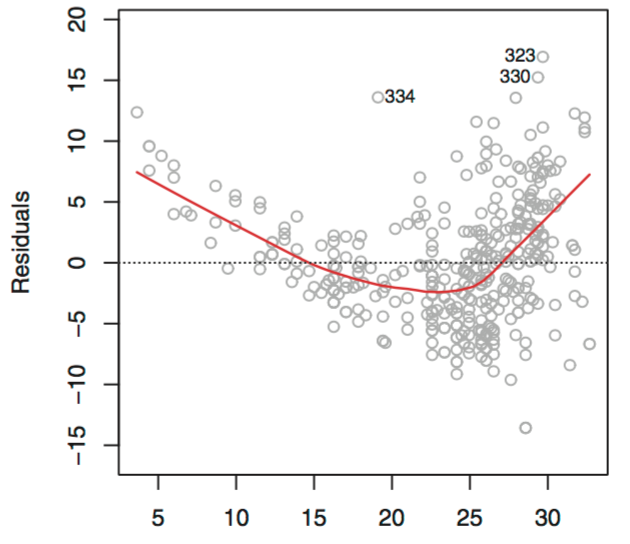
\includegraphics[width=1.725in]{stuff/resids.png}

\vspace{-.1in}
$\quad\quad\quad\quad\quad\quad\;\; X$}

\end{column}
\end{columns}


}


\frame
{
 \frametitle{Leverage\only<3>{: \textcolor{Maroon}{So}}\only<4>{: \textcolor{Maroon}{And now}} \only<3-4>{\textcolor{Maroon}{high or low leverage?}} }
The \emph{hat} matrix $H$ \emph{``puts the hat on''} ${\boldsymbol Y}$ \textcolor{gray}{projecting ${\boldsymbol Y}$ onto the (least squares) closest vector to ${\boldsymbol Y}$ in the column space of $\boldsymbol x, \hat {\boldsymbol Y} \in \mathcal{R}(\boldsymbol x)$  }

\begin{columns}
\begin{column}{.01\textwidth}
$\;$
\end{column}
\begin{column}{.275\textwidth}
\begin{align*}
\\{}\\
H = {} & \textbf{x}(\textbf{x}^T\textbf{x})^{-1}  \textbf{x}^T\\
\hat {\boldsymbol Y}  = {} & \textbf{x}(\textbf{x}^T\textbf{x})^{-1}  \textbf{x}^T\textbf{Y}\\
 = {} & H\textbf{Y}\\{}\\{}\\
\end{align*}
\end{column}
\begin{column}{.7\textwidth}
\only<3>{\hspace{.34em}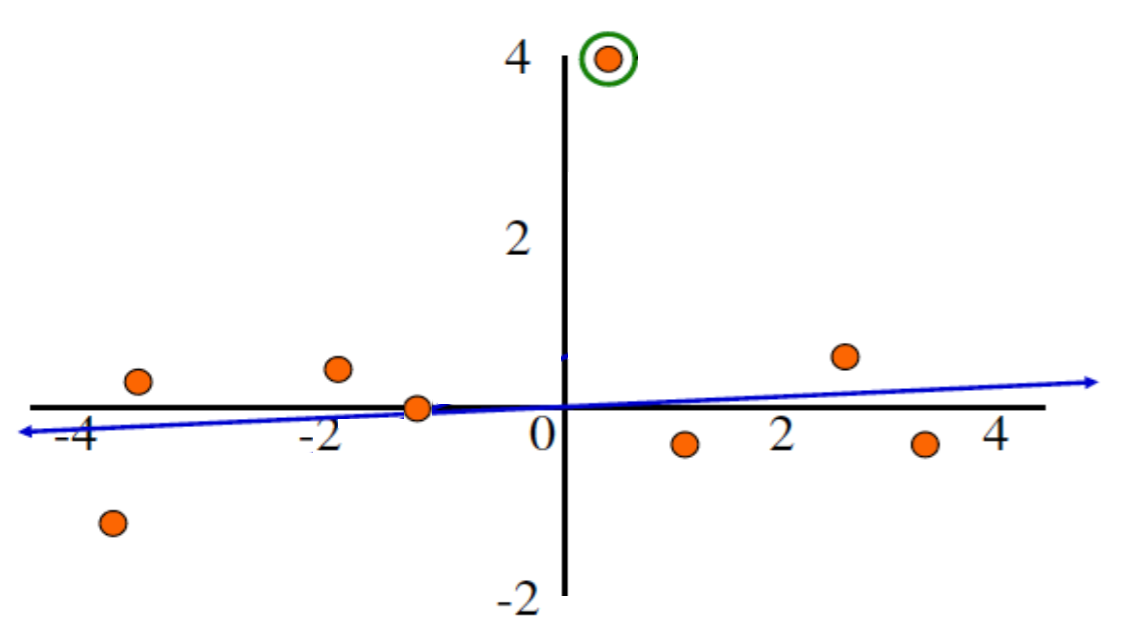
\includegraphics[width=2.75in]{stuff/outliers6.png}}
\only<4->{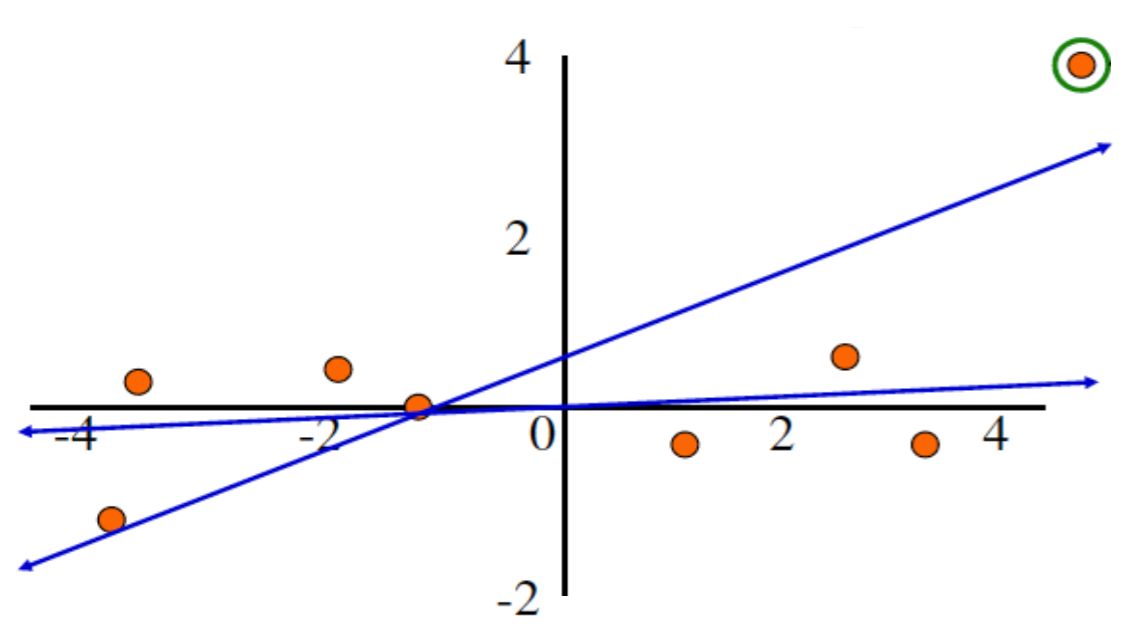
\includegraphics[width=2.75in]{stuff/outliers5.png}}\\${}$
\end{column}
\end{columns}

\vspace{-1.5em}
\begin{itemize}
\item<2-> Diagonal element $H_{ii} \in [0, 1]$, and $\sum_{i=1}^n H_{ii} = rank(\textbf{x})$
\item<2->[] \textcolor{gray}{$H_{ii}$ is called the \emph{leverage} of observation $i$}
\item<3-> $H_{ii}$ shows much $\hat Y_i$ depends on $Y_i$ 
\item<3->[] \textcolor{gray}{which depends on the ``extremeness'' of $x_i$} 
\item<5->  \textcolor{blue}{Relative comparison of $H_{ii}$'s id.'s ``high leverage observations'' }
\end{itemize}


}





\frame
{
 \frametitle{Influential Data Points}

%``Student's t-distributioned'' 

\begin{columns}
\begin{column}{.45\textwidth}

\textcolor{NavyBlue}{Studentized Residuals\\ have a t-distribution...}

$$ r_i = \frac{\hat \epsilon_i}{\hat \sigma \sqrt{1-h_{ii}} }$$ \\${}$\\${}$\\${}$


\onslide<2->{
\textcolor{Maroon}{Cook's Distance is}
\begin{align*}
D_i =& \frac{\sum_{j=1}^n \left(\hat y_j - \hat y_{j(-i)}\right)^2}{\hat \sigma^2p}\\
=& \frac{\hat \epsilon_i}{\hat \sigma^2p}\frac{h_{ii}}{(1-h_{ii})^2}
\end{align*}
}

\end{column}
\begin{column}{.55\textwidth}
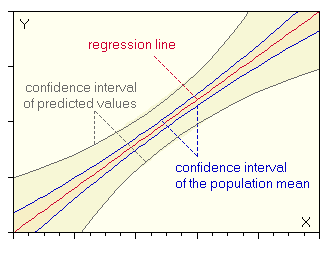
\includegraphics[width=2in]{stuff/hl_regress_confiv.png}

\onslide<2->\hspace{.5em}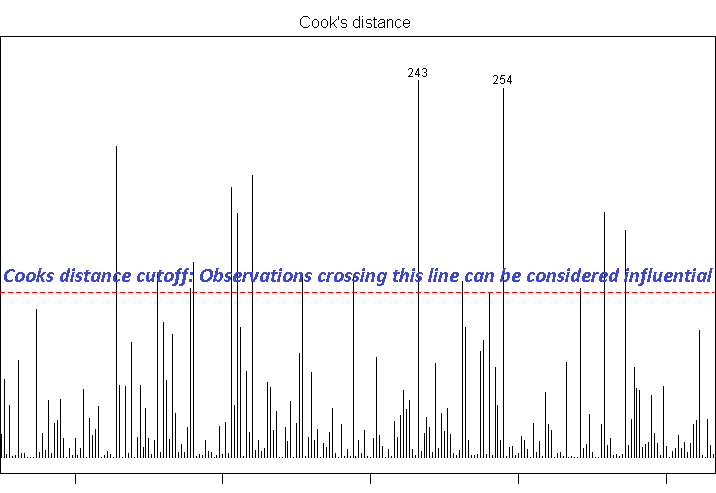
\includegraphics[width=1.9in]{stuff/cooks2.png}

\end{column}
\end{columns}

${}$\\
%\frac{\text{residual}_i}{\text{RSE}}

Influential data point $i$ may have $D_i >$ 
$\{ 3 \times \bar D, 1, 4/n, F_{p,n-p}^{1-\alpha}\}$


}



\frame
{
 \frametitle{Multivariate Regression}
 
% \scriptsize
%That seriously major transition that just happened that you didn't even notice?
 %\normalsize
 
 \vspace{-.11em}
 
\begin{align*}
Y_i = {}& \beta_0+\beta_1x_{i1} \textcolor{white}{ \;+ \cdots + \beta_p x_{ip}} + \epsilon_i,  \;  \epsilon_i \overset{\tiny i.i.d.}{\sim}  \textrm{N}(0,\sigma^2)\\{}\\
 {\boldsymbol Y} \sim {} &  \textrm{MVN}(\textbf{x}{\boldsymbol\beta},\sigma^2I)\\{}\\
\tiny
\left[\begin{array}{c} Y_1 \\ Y_2 \\ Y_3 \\ \vdots\\ Y_n \end{array} \right] 
= {} & \tiny{\Large \text{$MVN$}} \left(
\left[\begin{array}{ccccc} 1 & x_{11} & \textcolor{white}{x_{21}} &\textcolor{white}{\cdots} & \textcolor{white}{\hspace{.2em}x_{p1}}\\
1 & x_{12} & \textcolor{white}{x_{22}} & \textcolor{white}{\cdots} & \textcolor{white}{x_{p2}}\\ 
1 & x_{13} & \textcolor{white}{x_{23}} & \textcolor{white}{\cdots} & \textcolor{white}{x_{p3}}\\ 
\vdots & \vdots & \textcolor{white}{\vdots} & \textcolor{white}{\ddots} & \textcolor{white}{\vdots}\\ 
1 & x_{1n} & \textcolor{white}{x_{2n}} & \textcolor{white}{\cdots} & \textcolor{white}{x_{pn}}
 \end{array} \right]  
 \left[\begin{array}{c}\beta_0 \\ \beta_1 \\ \textcolor{white}{\beta_2} \\ \textcolor{white}{\vdots}\\ \textcolor{white}{\beta_p} \end{array} \right]_,
 \left[\begin{array}{cccc}\sigma^2&0 & \cdots & 0\\ 
0 &\sigma^2&  \cdots & 0\\
\vdots &\vdots&  \ddots & \vdots\\
0 & 0 &   \cdots & \sigma^2\\ \end{array}\right]\right)\end{align*}

\begin{itemize}
\item[]
\item<1-> Regression is a (multivariate) normal distribution 
\item[]<1-> with a \emph{linear model} component for the mean 
\item[]
\item[]

\end{itemize}

}



\frame
{
 \frametitle{Multivariate Regression}
 
% \scriptsize
%That seriously major transition that just happened that you didn't even notice?
 %\normalsize
 
\begin{align*}
Y_i = {}& \beta_0+\beta_1x_{i1} + \cdots + \beta_px_{ip} + \epsilon_i,  \;  \epsilon_i \overset{\tiny i.i.d.}{\sim}  \textrm{N}(0,\sigma^2)\\{}\\
 {\boldsymbol Y} \sim {} &  \textrm{MVN}(\textbf{x}{\boldsymbol\beta},\sigma^2I)\\{}\\
\tiny
\left[\begin{array}{c} Y_1 \\ Y_2 \\ Y_3 \\ \vdots\\ Y_n \end{array} \right] 
= {} & \tiny{\Large \text{$MVN$}} \left(
\left[\begin{array}{ccccc} 1 & x_{11} & x_{21} &\cdots & x_{p1}\\
1 & x_{12} & x_{22} & \cdots & x_{p2}\\ 
1 & x_{13} & x_{23} & \cdots & x_{p3}\\ 
\vdots & \vdots & \vdots & \ddots & \vdots\\ 
1 & x_{1n} & x_{2n} & \cdots & x_{pn}
 \end{array} \right]  
 \left[\begin{array}{c}\beta_0 \\ \beta_1 \\ \beta_2 \\ \vdots\\ \beta_p \end{array} \right]_,
 \left[\begin{array}{cccc}\sigma^2&0 & \cdots & 0\\ 
0 &\sigma^2&  \cdots & 0\\
\vdots &\vdots&  \ddots & \vdots\\
0 & 0 &   \cdots & \sigma^2\\ \end{array}\right]\right)\end{align*}

\begin{itemize}
\item[]
\item<1-> Regression is a (multivariate) normal distribution 
\item[]<1-> with a \emph{linear model} component for the mean 
\item[]
\item<2-> %$\text{E}[Y] = \beta_0 + \beta_1X_1 + \beta_2X_2 + \beta_{2^2}X_2^2 + \beta_{13}X_1X_3 $
\textcolor{red}{Interpret: ``vary one $X$ and hold all others constant''?}
\end{itemize}

}




\frame
{
 \frametitle{Assumptions, violations, and remedial measures}

\vspace{-1in}

$$Y_i = \beta_0+\beta_1x_{i1} + \cdots + \beta_px_{ip} + \epsilon_i,  \;  \epsilon_i \overset{\tiny i.i.d.}{\sim} \textrm{N}(0,\sigma^2)$$
 
\begin{columns}
\begin{column}{.33\textwidth}
\begin{itemize}
\item<2-> Normality
\item<4-> Homoskedasticity
\item<6-> Independence
\item<7-> Linear form
\item<8-> Fixed $x$'s
\end{itemize}
\end{column}
\begin{column}{.67\textwidth}
%\vspace{.25in}
\begin{itemize}
\item<2-3> [] 
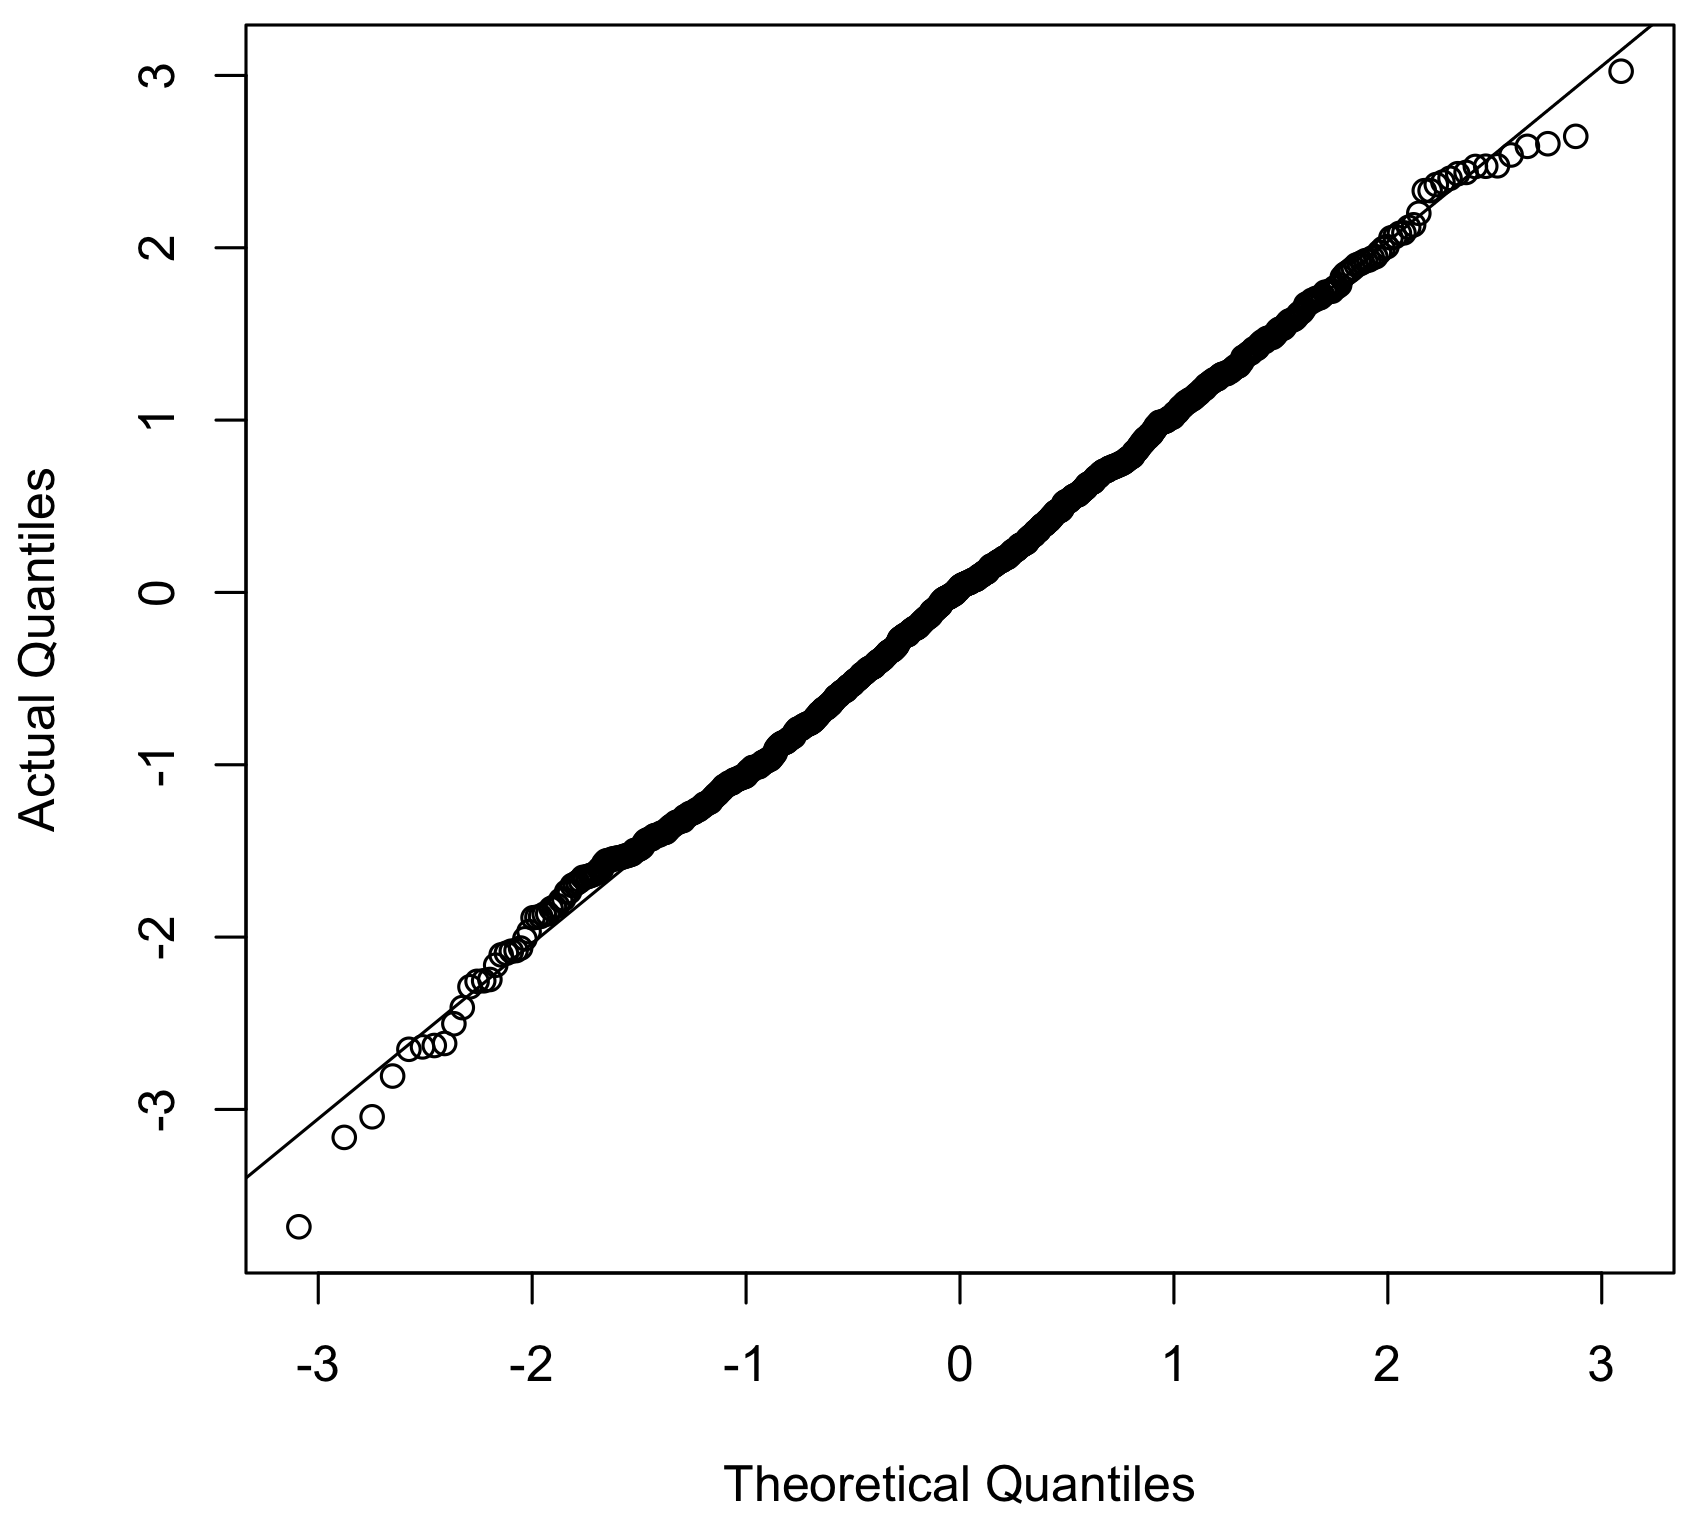
\includegraphics[width=2in]{stuff/qq1.png}\\ % statistical results compromised -- can perhaps transform
Q-Q Plot\\${}$\\
\textcolor{gray}{Hypothesis testing depends on distributional assumptions}
 % transform 
\vspace{-2.64in}
\item<2>[] 

\textcolor{white}{llllllll}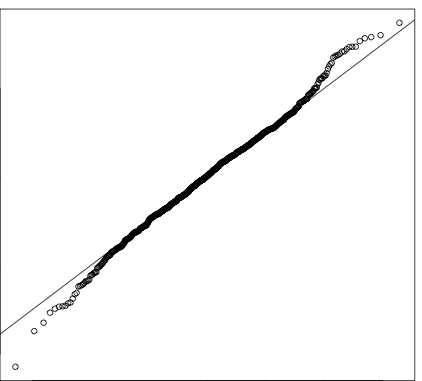
\includegraphics[width=1.715in,height=1.51in]{stuff/qq2.png}

\vspace{-1.7in}
\item<4-5> [] 
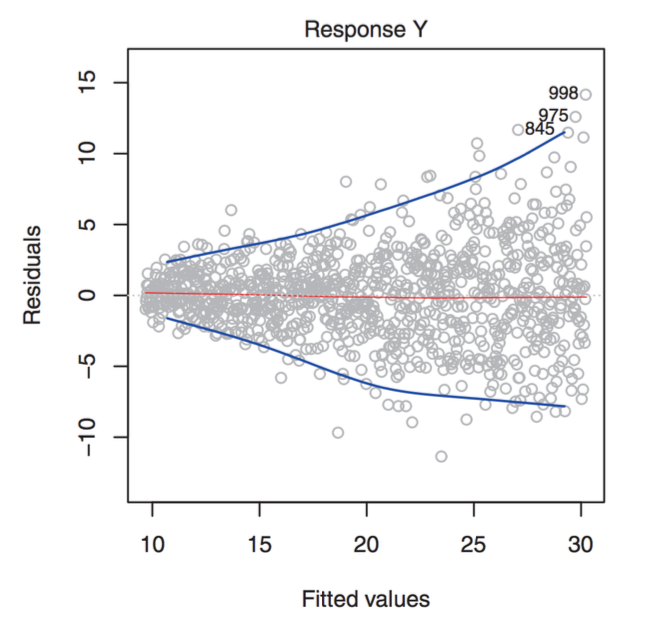
\includegraphics[width=2in]{stuff/hets1.png}\\ % statistical results compromised -- can perhaps transform
Residuals versus Fitted Values\\${}$\\
\textcolor{gray}{Box-Cox transformations $\frac{Y^\lambda-1}{\lambda}$ can help}
 % transform 
\vspace{-2.75in}
\item<5>[] 
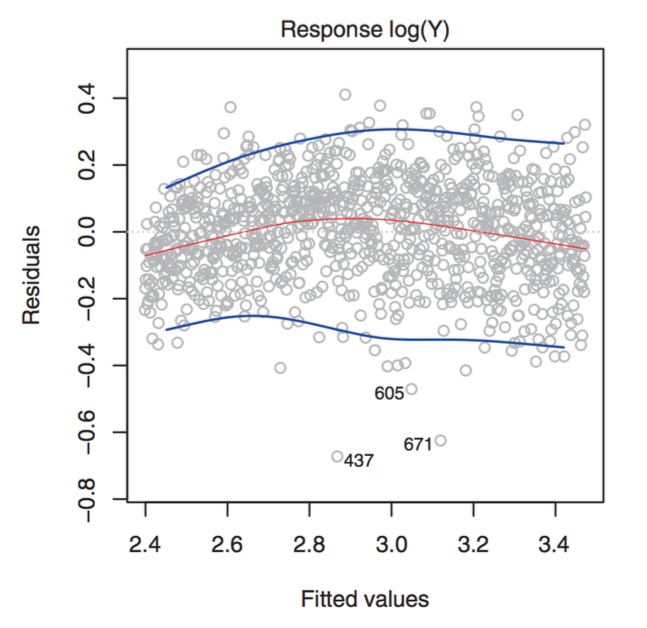
\includegraphics[width=2in]{stuff/hets2.png}
\item<6>[] 
\vspace{-1.5in}
$\text{Cov}[{\boldsymbol Y} - {\boldsymbol X\beta}]$
%= \frac{({\boldsymbol Y} - {\boldsymbol X\beta})({\boldsymbol Y} - {\boldsymbol X\beta})^T}{n-p-1}$\\${}$\\
%$\quad\quad\quad\quad\quad\quad
$\approx\left[\begin{array}{cccc}\sigma^2&0 & \cdots & 0\\ 
0 &\sigma^2&  \cdots & 0\\
\vdots &\vdots&  \ddots & \vdots\\
0 & 0 &  \cdots & \sigma^2\\ \end{array}\right]$

\item<7>[] 
\vspace{-1.25in}
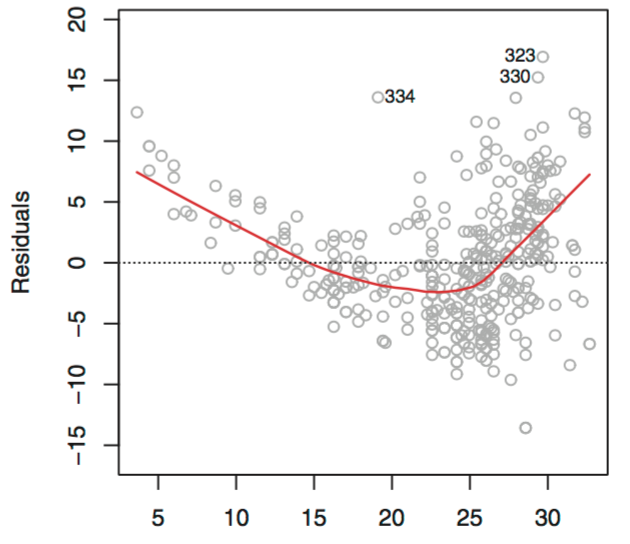
\includegraphics[width=2in]{stuff/resids.png}\\ % statistical results compromised -- can perhaps transform
Residuals versus Feature Values\\${}$\\
\textcolor{gray}{``All models are wrong, some are useful'' -- George Box}

\item<8>[]\huge 
\vspace{-2.5in}$${\boldsymbol Y} \sim  \textrm{MVN}(\textbf{x}{\boldsymbol\beta},\sigma^2I)$$

\end{itemize}
\end{column}
\end{columns}
%fits.png


% stats people care about diagnostics -- do you?
%\item Challenges interpreting coefficients? 

}




\frame
{
 \frametitle{Quiz: assumptions?}

$$Y_i = \beta_0+\beta_1x_{i1} + \cdots + \beta_px_{ip} + \epsilon_i,  \;  \epsilon_i \overset{\tiny i.i.d.}{\sim} \textrm{N}(0,\sigma^2)$$


\begin{enumerate}
\item
\item
\item
\item
\item
\item[]
\item<2->[] \tiny There are a number of ways these assumptions are characterized (i.e., differently in economics, e.g.) \\
\textbf{but this is how **I** want you to think about and remember and describe these assumptions}
\end{enumerate}

\large
\begin{itemize}
\footnotesize
\setlength\itemsep{.15em}
\color{red}
\item[]<3-> so we just spent all this time looking at diagnostics and \item[]
\item[]<3-> \huge \emph{Why care we so much this stuff??}
\end{itemize}

}



\frame
{
 \frametitle{Coefficients are Multivariate Normal (MVN)}
 
 \setlength{\leftmargini}{-10pt}

\begin{align*}
f(\textbf{Y}|\textbf{x},{\boldsymbol\beta}, \sigma^2) = {} & \prod_{i=1}^n f(Y_i|\textbf{x}_i,{\boldsymbol\beta}, \sigma^2) \\
\onslide<1->{= {} & \prod_{i=1}^n N(\textbf{x}_i^T{\boldsymbol\beta}, \sigma^2)} \\
\onslide<1->{= {} & \prod_{i=1}^n \frac{1}{\sqrt{2\pi \sigma^2}} e^{-\frac{1}{2\sigma^2}(Y_i-\textbf{x}_i^T{\boldsymbol\beta})^2}}\\
\onslide<1->{ = {} & (2\pi \sigma^2)^{-\frac{n}{2}} e^{-\frac{1}{2\sigma^2}(\textbf{Y} - \textbf{x}{\boldsymbol\beta})^T(\textbf{Y} - \textbf{x}{\boldsymbol\beta})} \;\; \textcolor{gray}{= MVN(\textbf{x}{\boldsymbol\beta},\sigma^2I)}} \\ {} \\
 \onslide<1->{\propto {} & e^{-\frac{1}{2\sigma^2}( (\textbf{x}^T\textbf{x})^{-1}  \textbf{x}^T\textbf{Y} - {\boldsymbol\beta})^T \textbf{x}^T\textbf{x} ( (\textbf{x}^T\textbf{x})^{-1}  \textbf{x}^T\textbf{Y} - {\boldsymbol\beta})}}\\ 
 \onslide<1->{= {} & e^{-\frac{1}{2\sigma^2}( \hat {\boldsymbol\beta} -   {\boldsymbol\beta})^T \textbf{x}^T\textbf{x} ( \hat {\boldsymbol\beta} -   {\boldsymbol\beta})}}\\ 
 \onslide<1->{\Longrightarrow {} & f(\hat {\boldsymbol\beta} |\textbf{x}, {\boldsymbol\beta}, \sigma^2) = MVN\left({\boldsymbol\beta},\sigma^2(\textbf{x}^T\textbf{x})^{-1}\right)} \\
\end{align*} 
}






\frame
{
 \frametitle{Multicollinearity and the Variance Inflation Factor (VIF)}

\onslide<1->{\textcolor{gray}{And when you have any number of covariates (features)...}}

\begin{itemize}
\item[] 
$$\hat {\boldsymbol\beta} \sim MVN\left({\boldsymbol\beta},\sigma^2(\textbf{x}^T\textbf{x})^{-1}\right)$$
\item<2>[] 
\begin{figure}
\centering
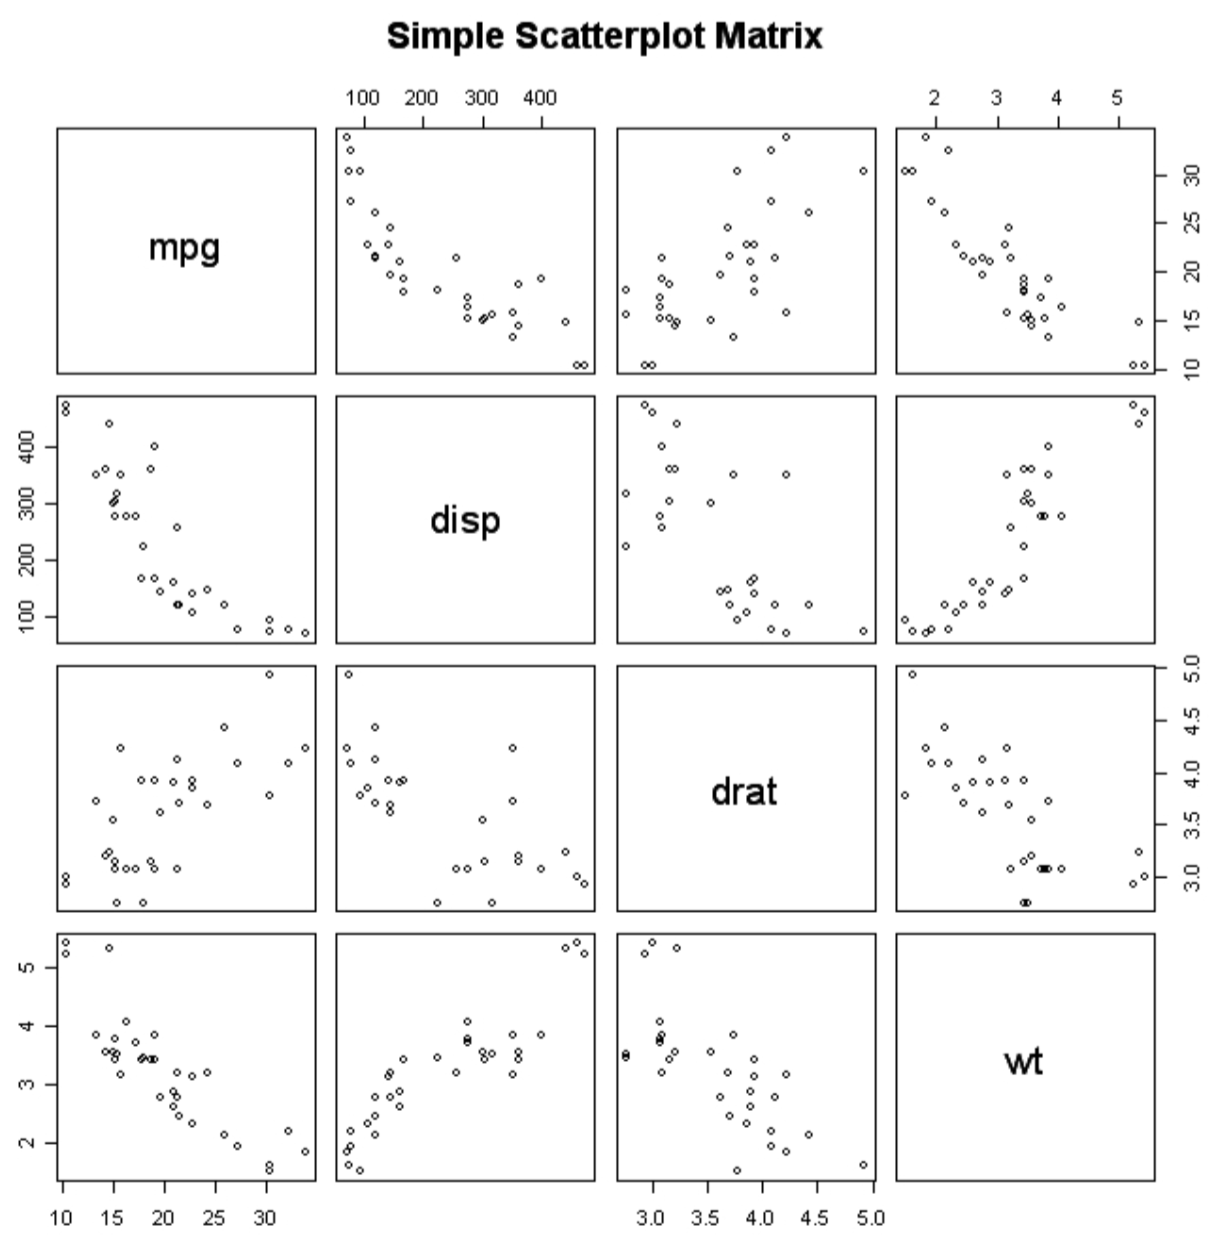
\includegraphics[width=2.4in]{stuff/VIF2.png}
\end{figure}
\vspace{-2.5in}
\item<3>[] 
\begin{figure}
\centering
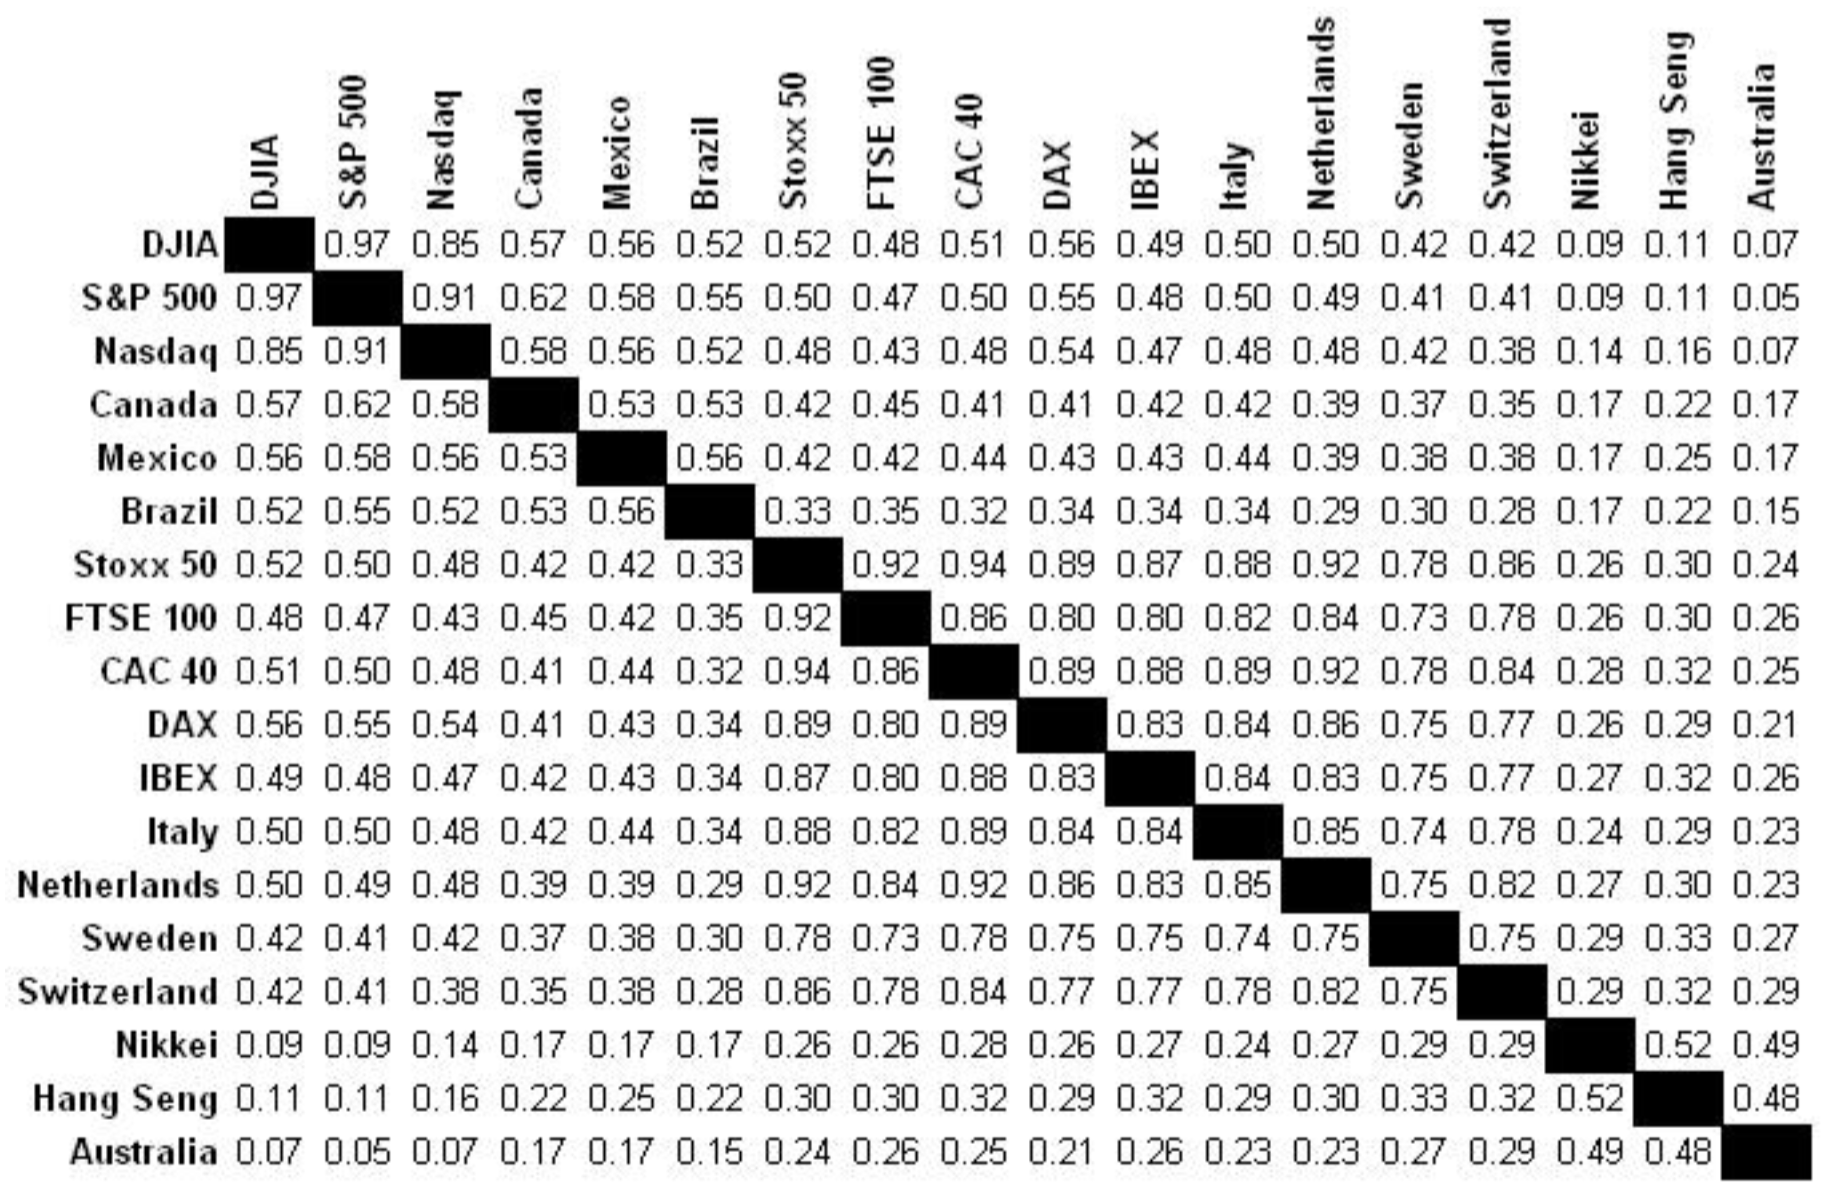
\includegraphics[width=3.5in]{stuff/VIF1.png}
\end{figure}
\vspace{-2.25in}
\item<4->[]${}$\\

 $$\widehat{\text{Var}}[\hat \beta_j] = \frac{\hat \sigma^2}{(n-1)  \widehat{\text{Var}}[X_j]}\cdot \textcolor{red}{\frac{1}{1-R^2_j}} \quad\quad \textcolor{red}{\text{[VIF]}}$$ 

where $R^2_j$ is the $R^2$ of $X_j$ regressed on all the other $X$'s\\${}$\\

\item<5->[] \textcolor{gray}{Could make an array of VIFs...?}

\end{itemize}


\footnotesize
${}$\\
${}$\\
\onslide<6->{\textcolor{gray}{Centering $X$'s can decorrelate $X$ and $X^2$...}}\\
\onslide<7->{\textcolor{gray}{Scaling $X$'s (to the same scale) numerically stabilizes the condition number}}

%\item The role of rank($X$) and multicollinearity? % centering/scaling

}


\frame
{
 \frametitle{Half time}
}











\frame
{
\frametitle{Assessing Model Fit \textbf{(more Machine Learning-ish)}}


\begin{table}[h!]
\centering
\begin{tabular}{|c|c|}
\hline
&\\
 Residual Sum of Squares  & Total Sum of Squares  \\
&\\
$RSS = \sum(Y_i - \hat Y_i)^2 \textcolor{gray}{= \sum \hat \epsilon_i^2}$ & $TSS = \sum(Y_i - \bar Y)^2 $ \\
 & $\textcolor{white}{RSEEEEEee}  \textcolor{gray}{= \sum( \hat Y_i - \bar Y )^2 + RSS}$ \\
&\\ \hline
&\\
Residual Standard Deviation & Proportion of Variance Explained\\
&\\
$\hat \sigma = \sqrt{\frac{1}{n-p-1}RSS}$ & $R^2 = \frac{TSS - RSS}{TSS}$ \\
$\textcolor{white}{RSEEEE} = \sqrt{\frac{\sum(Y_i - \hat Y_i)^2}{n-p-1}}$ &$\textcolor{white}{R} = 1-\frac{RSS}{TSS}$\\
&\\ \hline
\multicolumn{2}{|c|}{$F$-statistic}\\
\multicolumn{2}{|c|}{$F =  \frac{(TSS - RSS)/p}{RSS/(n-p-1)} = \frac{\sum(\hat Y_i -\bar Y )^2/p}{\sum( Y_i -\hat Y )^2/(n-p-1)}$}\\ 
\multicolumn{2}{|c|}{${}$}\\\hline
\end{tabular}
\end{table}

}

\frame
{
 \frametitle{Decomposition of Total Variation}

\begin{figure}
\centering
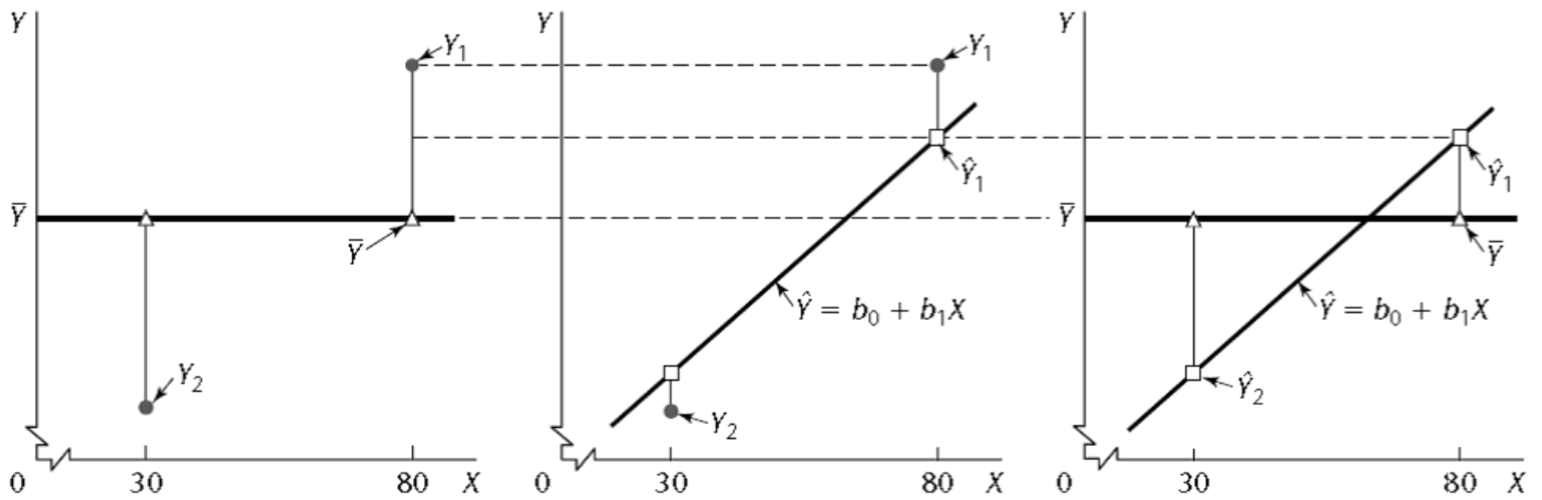
\includegraphics[width=4in]{stuff/sspartition.png} 
\end{figure}
\vspace{-2em}

\begin{align*}
TSS = {} & \sum(Y_i - \bar Y)^2 =  \sum( Y_i - \hat Y_i + \hat Y_i - \bar Y )^2 \\
= {} & \sum( Y_i - \hat Y_i )^2 + 2 \sum ( Y_i - \hat Y_i )( \hat Y_i - \bar Y ) +\sum( \hat Y_i - \bar Y )^2 \\
= {} & \sum( Y_i - \hat Y_i )^2 + 2 \sum \hat \epsilon_i ( \hat Y_i - \bar Y ) + \sum( \hat Y_i - \bar Y )^2 \\
{} &\textcolor{gray}{\quad\quad\quad\quad\quad\sum \hat \epsilon_i = 0 \uparrow \;\;\; \uparrow \sum \hat \epsilon_i\hat Y_i = 0}\\
= {} & \sum( Y_i - \hat Y_i )^2 + \sum( \hat Y_i - \bar Y )^2 =  RSS + \sum( \hat Y_i - \bar Y )^2 
\end{align*}

}


\frame
{
 \frametitle{MODEL SELECTION!!!}

\begin{itemize}
\item<1-> $R^2$ (model fit) is insufficient -- more features means larger $R^2$
\item<2-> Spuriously improving model fit to data is called \emph{overfitting}
\item<3-> \underline{We want model fits to generalize to \emph{population} phenomenon} 
\item[]
\item<4-> Classical Statistics Approaches: 
\item[]<4-> Model Selection Criterion (choose smallest)\\${}$\\
\begin{tabular}{|rl|l|}
\hline & &\\
Mallow's $C_p$ & $\frac{1}{n}(RSS + 2p\hat\sigma^2)$ & \\
&&\\
$AIC$ & $-2\log L+2p$          & $D_M = - 2\text{log}f(Y|\hat \theta^{M_p})$ \\
&                                            &  $ \textcolor{white}{D_M = } + 2\text{log}f(Y|Y)$ \\             
$BIC$ & $-2\log L+p\log n $  & \\
&&\textcolor{gray}{$D_M \overset{\tiny approx.}{\sim}   \chi^2_{n-p-1}$} \\
$Adjusted \; R^2$ & $1 - \frac{RSS/(n-p-1)}{TSS/(n-1)}$& \\
&&\\\hline 
\end{tabular}
\end{itemize}

}



\frame
{
\frametitle{Assessing Parameter Uncertainty \textbf{(definitely Statistics)}}
 
For $\hat{\boldsymbol\beta}  = (\textbf{x}^T\textbf{x})^{-1}  \textbf{x}^T\textbf{Y}$, since (under $H_0$)
$$f(\hat {\boldsymbol\beta} | {\boldsymbol\beta}, \sigma^2, \textbf{x}) = MVN\left({\boldsymbol\beta}, \sigma^2(\textbf{x}^T \textbf{x})^{-1}\right)$$
we have that 
\onslide<2->{$$\frac{\hat \beta_i - \beta_i}{\text{SD}(\hat \beta_i)} \sim  N(0,1)$$}
\onslide<3->{and if we estimate 
$$\hat \sigma^2 = \frac{(\textbf{Y} - \textbf{x}\hat{\boldsymbol \beta})^T(\textbf{Y} - \textbf{x}\hat{ \boldsymbol  \beta})}{n-p-1} = \frac{\sum_{i=1}^n \hat \epsilon_i^2}{n-p-1} $$
(where $p$ is the number of coefficients) then we have that} 
\onslide<4->{$$\frac{\hat \beta_i - \beta_i}{\widehat{\text{SD}}(\hat \beta_i)} \sim  t_{n-p-1}$$}
\vspace{-.25em}
\onslide<4->{\textcolor{gray}{And this works for any number of feature variables...}}
%\left({\boldsymbol\beta}

}



\frame
{
 \frametitle{Hypothesis Testing for Feature Selection}

\vspace{-1em}
\begin{align*}
\textcolor{gray}{F =} {}& \textcolor{gray}{\frac{(TSS - RSS)/p}{RSS/(n-p-1)} = \frac{\sum(\hat Y_i -\bar Y )^2/p}{\sum( Y_i -\hat Y )/(n-p-1)}} \\{}\\
F \sim  {}& F_{p,n-p-1} \quad \textcolor{gray}{\text{(tests if any coefficient is \emph{non-zero})}} \\ 
\frac{\hat \beta_i - \beta_i}{\widehat{\text{SD}}(\hat \beta_i)} \sim  {} & t_{n-p-1} \quad\quad \textcolor{gray}{\text{(tests if a \emph{specific} coefficient is non-zero*)}}\\
{} &\;\quad\quad\quad\quad \scriptsize \textcolor{gray}{\text{*in the presence of all the others (this is a ``last-in'' test)}}\\
\end{align*}

\vspace{-.6in}
\begin{itemize}
\item<2->[]
\hspace*{.75in}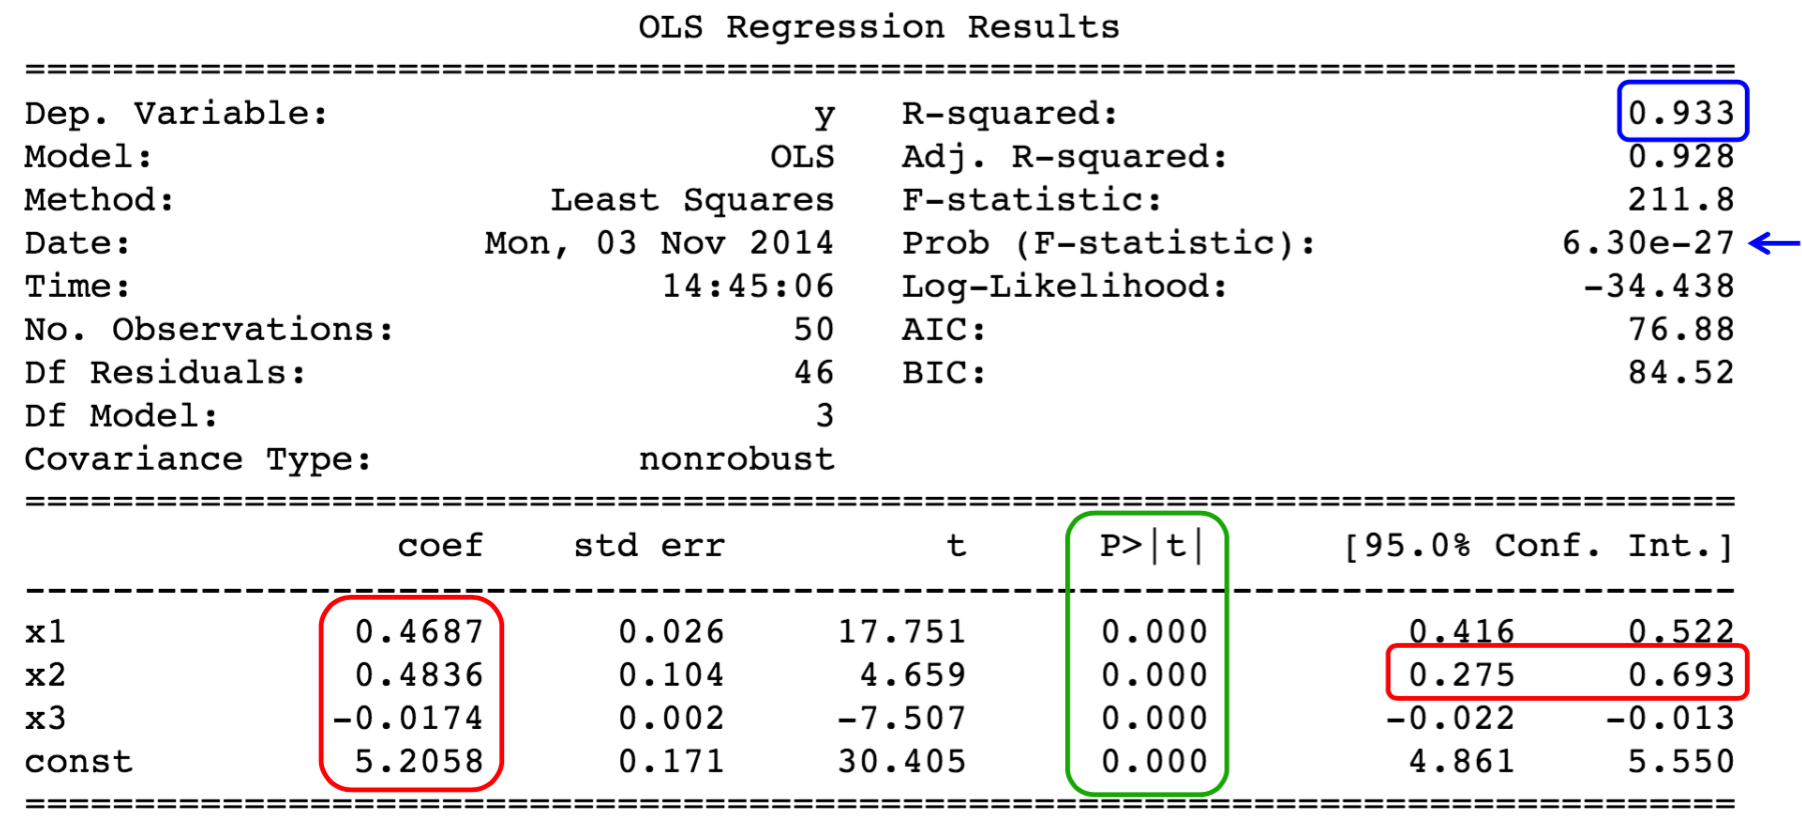
\includegraphics[width=3.5in]{stuff/regtable.png} 
\vspace{-1.6in}
\item<3-> Forward \\Selection\\${}$\\
\item<4-> Backward \\Selection\\${}$\\
\item<5-> Both \\${}$\\
\end{itemize}


}


\frame
{
 \frametitle{Testing: \emph{other flavors}}

\vspace{-.1in}

${}$\\${}$\\${}$\\${}$\\
\begin{columns}
\begin{column}{.6\textwidth}
\fbox{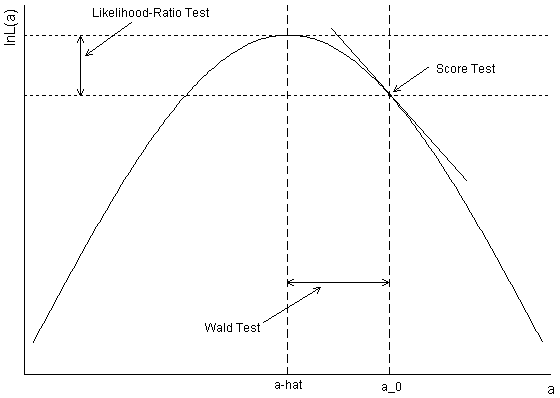
\includegraphics[width=2.3in]{stuff/waldVS.png}}
\end{column}
\begin{column}{.55\textwidth}
\vspace{-.075in}

\underline{Wald test}\\
$\sqrt{\frac{(\hat \theta - \theta_0)^2}{Var(\hat \theta)}} \overset{\tiny approx.}{\sim} N(0,1) \textcolor{gray}{\text{ under } H_0}$\\${}$

\underline{Likelihood-Ratio (LR) test}\\
$-2ln\left(\frac{L(\theta_0|x)}{{L(\theta|x)}}\right) \overset{\tiny approx.}{\sim} \chi^2_k \textcolor{gray}{\text{ under } H_0}$\\${}$

\underline{Score test} \\
$\frac{\left(\frac{\partial}{\partial \theta } \log L(\theta_0|x)\right)^2}
{-\text{E}\left[\frac{\partial^2}{\partial \theta^2 } \log L(\theta_0|x)\right]} \overset{\tiny approx.}{\sim} \chi^2_1 \textcolor{gray}{\text{ under } H_0}$

\end{column}


\end{columns}
${}$\\${}$\\${}$\\${}$\\
\onslide<1->{\hspace{.35em}\textcolor{gray}{And this works for any number of feature variables...}}

}






\frame
{
 \frametitle{Testing: \emph{demonstrated in simple linear regression}}
 
 
 \setlength{\leftmargini}{-10pt}
\vspace{-1.5em}
\begin{itemize}
\color{gray}
\item[] 
\begin{align*} 
f(\textbf{Y}|{\textbf{x}, \boldsymbol\beta}, \sigma^2) = {} & MVN(\textbf{x}{\boldsymbol\beta},\sigma^2I) \\
 \Longrightarrow f(\hat {\boldsymbol\beta} | \textbf{x}, {\boldsymbol\beta}, \sigma^2) = {} & MVN\left({\boldsymbol\beta},\sigma^2(\textbf{x}^T\textbf{x})^{-1}\right) 
\end{align*} 

\color{black}

\item[]<1-> For simple linear regression then 

$$\hat {\boldsymbol\beta} \sim MVN\left( \left[\begin{array}{c} \beta_0 \\ \beta_1 \end{array}\right]_{\Large,} 
\frac{\sigma^2}{n \sum (x_i - \bar x)^2} \left[\begin{array}{cc} \sum x_i^2 & - \sum x_i\\ - \sum x_i&  n \end{array} \right] \right) $$

\item[]<1->
where 

$$\textcolor{gray}{\hat \beta_0 = \bar Y -  \hat \beta_1 \bar x \quad
\hat \beta_1 = \frac{\sum_{i=1}^n (Y_i - \bar Y) (x_i - \bar x)}{\sum_{i=1}^n (x_i - \bar x)^2} = \frac{R_{xY}S_Y}{S_x}}$$

$$\text{Var}(\hat \beta_1) = \sigma^2\frac{1}{\sum_{i=1}^n (x_i - \bar x)^2} \quad
\text{Var}(\hat \beta_0) = \sigma^2\left[\frac{1}{n} + \frac{\bar x^2}{\sum_{i=1}^n (x_i - \bar x)^2} \right]$$
%\vspace{.1em}

\item[]<1-> 
$$\textcolor{gray}{\text{SD}(\hat \beta_0) = \sqrt{\text{Var}(\hat \beta_0)} \quad \text{SD}(\hat \beta_1) = \sqrt{\text{Var}(\hat \beta_1)}}$$
\end{itemize}
}




\frame
{
 \frametitle{Testing: \emph{extra credit}}

\begin{itemize}
\item
What is $\text{Var}(\hat Y_0)$? \textcolor{gray}{(Suppose we know $\sigma^2$)}
%\item[] % use general variance formula
%\item[] % get (\sigma^2/n)*(sum(x_i-x_0)^2/sum(x_i-\bar x)^2) 
%\item[] % and can also show (with the other formula) that 
%\item[] % get \sigma^2(1/n + (x_0 - \bar)x^2/sum(x_i-\bar x)^2]
\item[] 
\item[] \emph{Hint: $\hat Y_0 = \hat \beta_0 +  x_0\hat \beta_1  $}
\item[] \emph{Hint: $\text{Var}[aX+bY]=\;?$}
\item[]
\item[]
\item[] 
\item
$\text{Var}(Y_0)$? For a \emph{new observation} $Y_0$ according to our model? 
\item[] \textcolor{gray}{(Suppose we know $\sigma^2$)}
\item[] 
\item \emph{Hint: $Y_0 = \hat \beta_0 +  \hat \beta_1 x_0 + \epsilon$}
\end{itemize}
}








\frame
{
 \frametitle{Linear Models}

\begin{itemize}
\item Linear model... that sounds too simple...
\item<2->[] 
\hspace*{-.25in}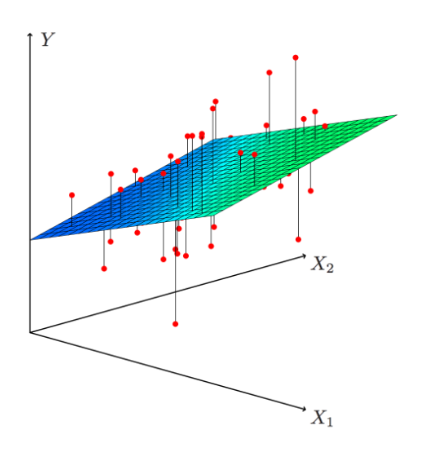
\includegraphics[width=1.75in]{stuff/OLS2.png}
\vspace{-1.75in}
\item<3->[] 
\hspace{1.4in}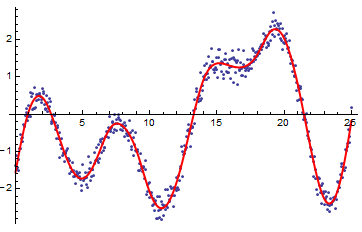
\includegraphics[width=2.5in]{stuff/spline.png} 
\item[] 
\item<4-> ``Linear'' models are only linear in the coefficients
$$Y_i = \beta_0+\beta_1x_{i1} + \cdots + \beta_px_{ip} + \epsilon_i$$
\item<4-> The $x$'s can be pretty wild... 
\end{itemize}

}




\frame
{
 \frametitle{Features that produce ``non-linear'' response surfaces?}
 
\begin{itemize}
\item<2-> Higher order terms: $X_1^{\frac{1}{2}},X_1^2, X_1^3$
\item<3-> Qualitative variables: $X_1 \in \{0,1\}, X_1 \in \{a,b,c,d\}$
\vspace{-.1in}
\item[]<4-> $$ \left[ \begin{array}{c}a\\b\\c\\d\end{array} \right] = \left[ \begin{array}{ccc}0&0&0\\1&0&0\\0&1&0\\0&0&1\end{array} \right] \quad\quad \left[ \begin{array}{c}a\\b\\c\\d\end{array} \right] \textcolor{red}{\not = \left[ \begin{array}{cccc}1&0&0&0\\0&1&0&0\\
0&0&1&0\\0&0&0&1\end{array} \right]} $$


\item<5-> Interactions: $X_1\cdot X_2$ \textcolor{gray}{\emph{$ + \; X_1 + X_2$ (interpretation?)}}
\item<6-> Step functions
\item[]<6> ${}$\\$Y_i = \beta_j : if \; a_j \leq X_i < b_j$
\item[]<6> 
\vspace{-.7in}
\hspace*{2in}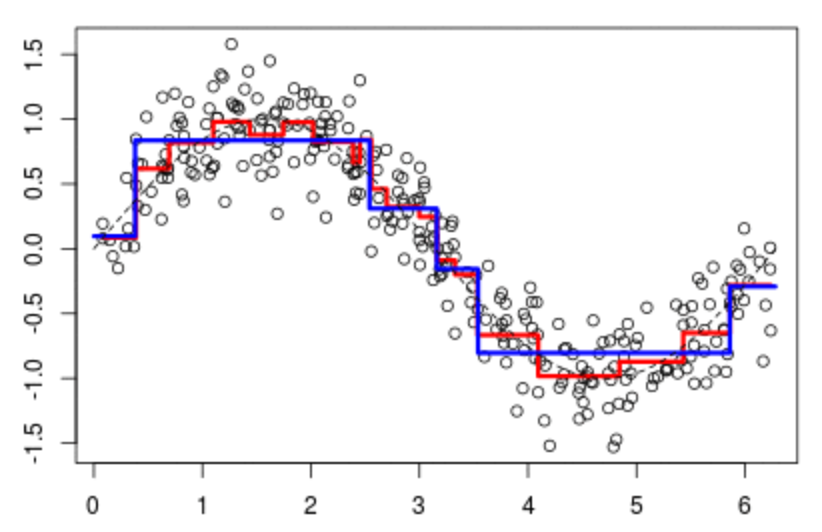
\includegraphics[width=2in]{stuff/step.png} 

\vspace{-1.175in}
\item<7-> Regression Splines\\${}$\\
\item[]<7> 
\vspace{.45in}
\hspace*{.0in}$Y_i = \left\{\begin{array}{ll} 
\beta_0 + \beta_1X_i + \beta_2X_i^2  +    \epsilon_i  : if  \; X_i \leq c\\
\beta_0^* + \beta_1X_i + \beta_2^*X_i^2  +  \epsilon_i  : if \; X_i > c
\end{array} \right. $
\item[]<7-8> 
\vspace{-1.4in}
\hspace*{2in}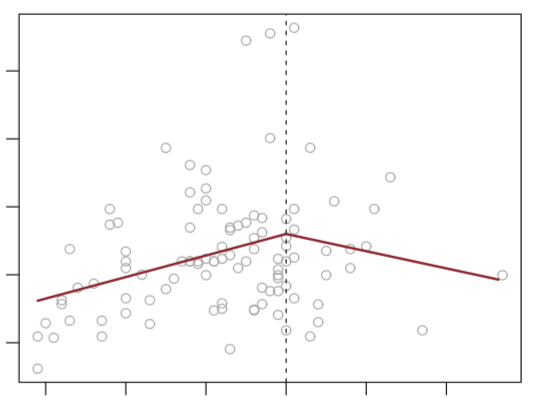
\includegraphics[width=1in]{stuff/splines1.png}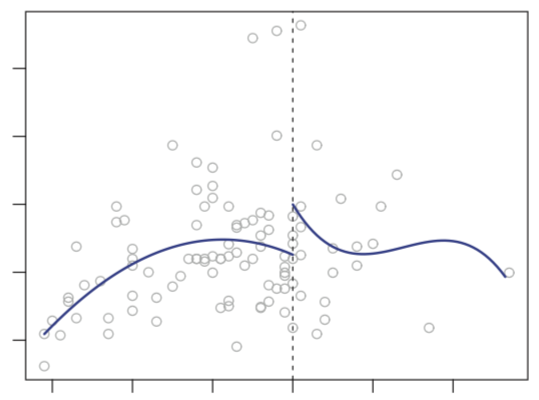
\includegraphics[width=1in]{stuff/splines2.png}

\onslide<8->{\hspace*{2in}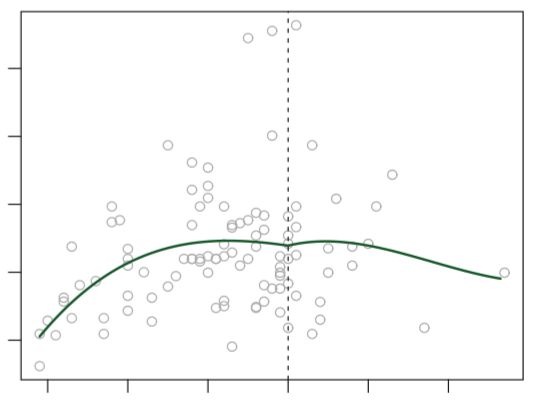
\includegraphics[width=1in]{stuff/splines3.png}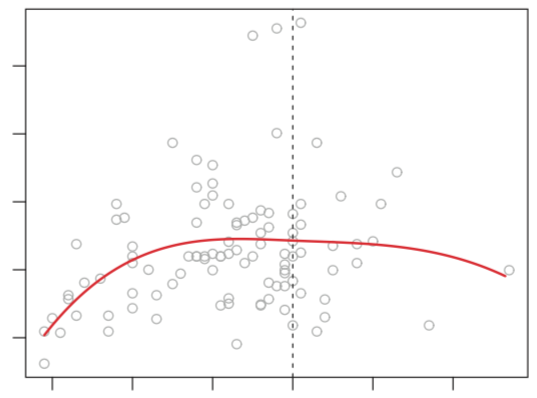
\includegraphics[width=1in]{stuff/splines4.png}} 
\item[]<8> 
\vspace{-1in}
\hspace*{-.525in}$h(X_i,\xi) = \left\{\begin{array}{ll} 
(x - \xi)^3 &:  if \; X_i > \xi \\
0 & :  if  \; X_i \leq \xi 
\end{array} \right.$  

$\quad$ \textcolor{gray}{\emph{basis functions} \& \emph{knots}}\\

\vspace{1em}

\hspace*{-.175in}$Y_i = \begin{array}{ll} 
\beta_0 + \beta_1X_i + \beta_2X_i^2  + \beta_3X_i^3   \\
+ \beta_{s1} h(X_i,\xi_1)  + \cdots + \epsilon_i 
\end{array} $
\vspace{-.63in}


\vspace{1in}


\end{itemize}
 
 %interpretation 
 
% \item Higher order terms -- what does ``linear'' mean? 
% indicator variabales
% interactions

% fancy polynomial splines
% smoothing splines
 
}

\frame
{
\frametitle{Linear models aren't really so ``linear''}

}


\frame
{
 \frametitle{Other ways to get ``non linear regressions''}
 
 
 
 \begin{itemize}
 
  \item Smoothing Splines  

\begin{figure}
\centering
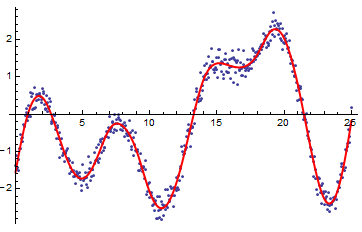
\includegraphics[width=3in]{stuff/spline.png} 

$\displaystyle\underset{g}{\min} \sum_{i=1}^n (Y_i -g(x_i))^2 + \lambda \int g''(t)^2 dt$
\end{figure}

\end{itemize}
}

\frame
{
 \frametitle{Other ways to get ``non linear regressions''}
 \begin{itemize}
 
 \item Local Regression (LOESS)
\begin{figure}
\centering
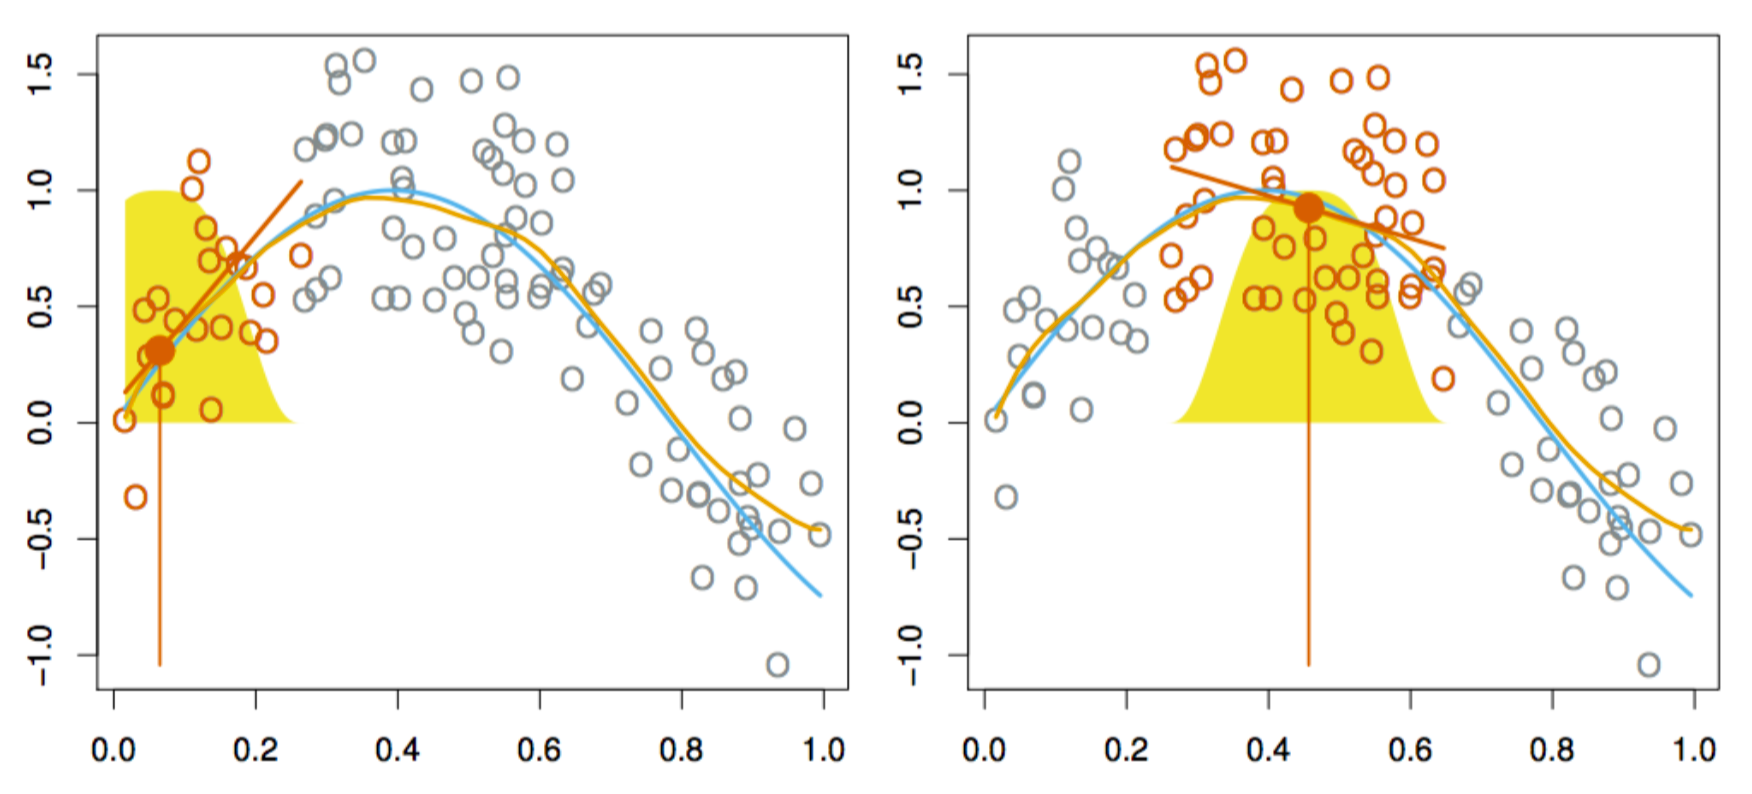
\includegraphics[width=4in]{stuff/loess.png} 
\end{figure}

\end{itemize}
}

\frame
{
 \frametitle{Other ways to get ``non linear regressions''}
 \begin{itemize}


 \item Generalized Additive Models
 
\begin{figure}
\centering
 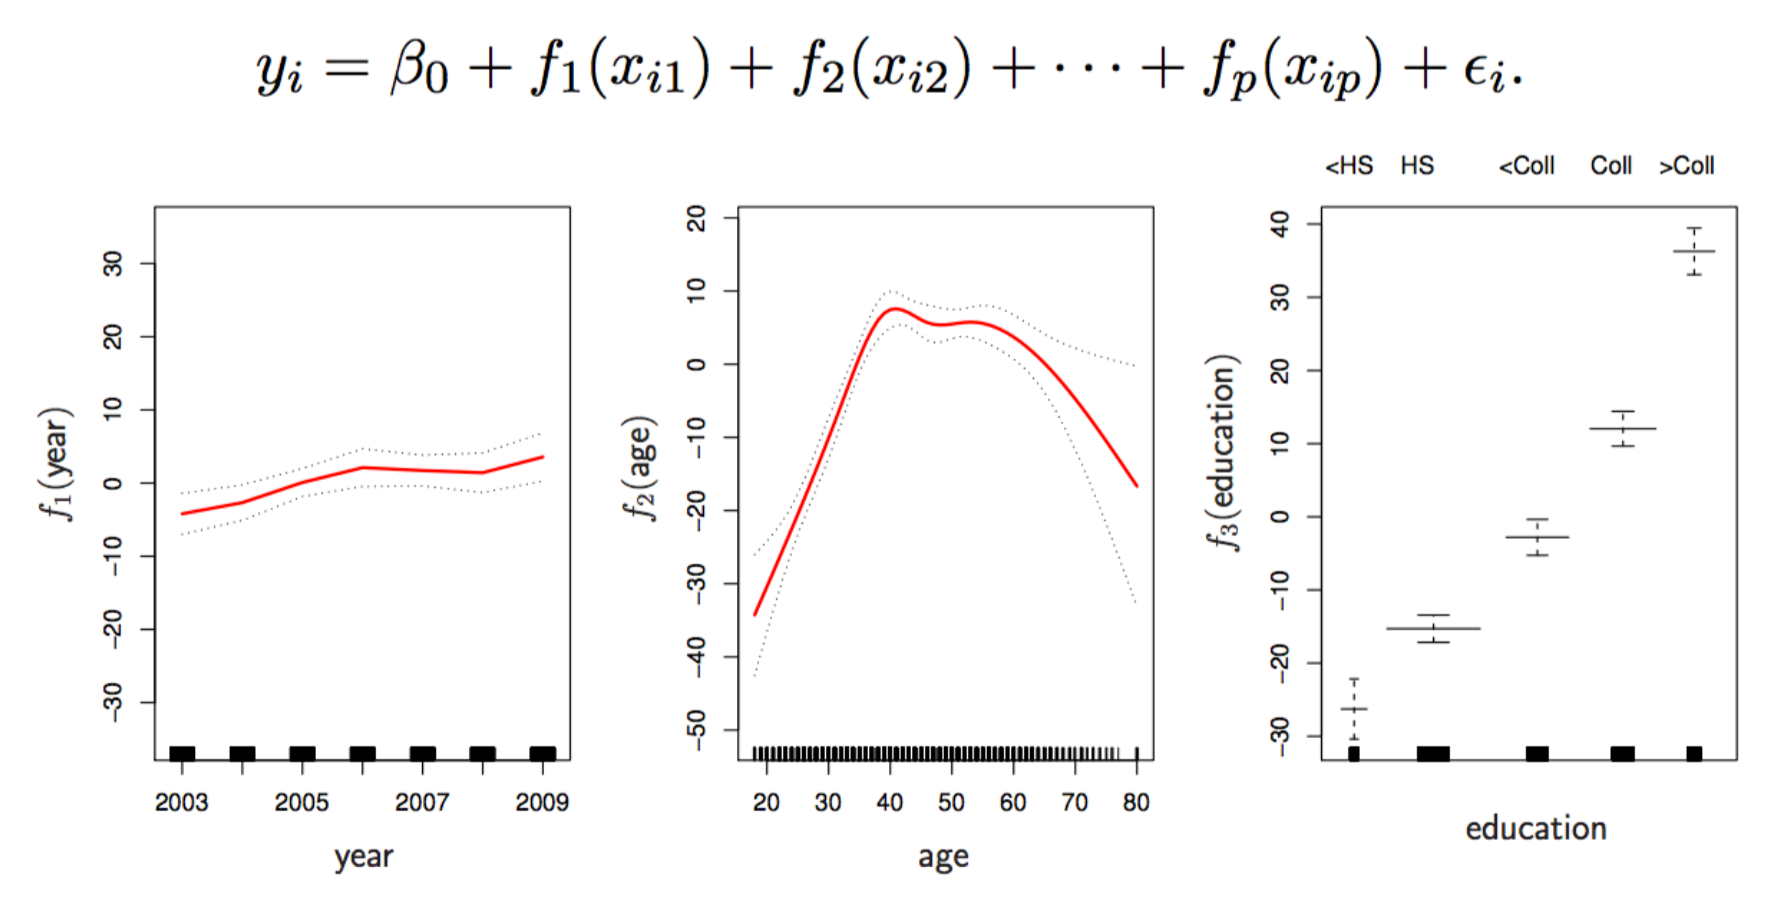
\includegraphics[width=4in]{stuff/gam.png} 

\end{figure}

 \end{itemize}
 
}


\end{document}








\frame
{
 \frametitle{Variance Partitioning and the Variance/Bias Tradeoff}
 
 \footnotesize
For fixed $\hat f(x)$ estimating true $f(x)$
\begin{align*}
\underset{Y}{\text{E}}[(Y-\hat f(x))^2] = {} & \underset{\epsilon}{\text{E}} [(f(x) + \epsilon - \hat f(x))^2] \\
= {} & \underset{\epsilon}{\text{E}} [(f(x) - \hat f(x) + \epsilon)^2 ] \\ 
= {} & \underset{\epsilon}{\text{E}} [(f(x) - \hat f(x))^2] + \underset{\epsilon}{\text{E}} [2(f(x) - \hat f(x))\epsilon]  + \underset{\epsilon}{\text{E}}[\epsilon^2]  \\ 
= {} & (f(x) - \hat f(x))^2 + 2(f(x) - \hat f(x))\underset{\epsilon}{\text{E}} [\epsilon]  + \underset{\epsilon}{\text{E}}[\epsilon^2]  \\ 
= {} & (f(x) - \hat f(x))^2 + \underset{\epsilon}{\text{E}}[\epsilon^2]  \\ 
{} & \quad reducible \quad\; irreducible \\
 reducible \quad\quad\quad\;\;&\\
 \underset{\hat f(x)}{\text{E}}\left[(f(x) - \hat f(x))^2\right] = {} & \underset{\hat f(x)}{\text{E}}\left[\left(f(x) - \underset{\hat f(x)}{\text{E}}[\hat f(x)] + \underset{\hat f(x)}{\text{E}}[\hat f(x)] - \hat f(x)\right)^2\right] \\
= {} & \underset{\hat f(x)}{\text{E}} \left[\left(f(x) - \underset{\hat f(x)}{\text{E}}[\hat f(x)] \right)^2\right] 
 +  \underset{\hat f(x)}{\text{E}}\left[\left(\underset{\hat f(x)}{\text{E}}[\hat f(x)] - \hat f(x)\right)^2\right] \\
& \quad\quad\quad\quad\quad\quad bias \quad\quad\quad\quad\quad\quad\quad\quad\quad variance  \\
\end{align*}
}






